\documentclass[12pt,a3paper]{article}
%  


%% ── Packages ──────────────────────────────────────────────────────────
\usepackage{amsmath,amssymb}
\usepackage{geometry}
\usepackage{enumitem}
\usepackage{titlesec}
\usepackage[hidelinks,colorlinks=true,linkcolor=blue!70!black]{hyperref}
\usepackage{xcolor}
\usepackage{fancyhdr}
\usepackage{tcolorbox}
\usepackage{multicol}
\usepackage{needspace}
\usepackage[strings]{underscore}
\usepackage{array,booktabs}
\usepackage[american]{circuitikz}
\tcbuselibrary{skins,breakable}
\geometry{margin=2.5cm,headheight=20pt,top=3cm,bottom=3cm}

%% ── Colors ────────────────────────────────────────────────────────────
\definecolor{pblue}{RGB}{13,71,161}
\definecolor{dgray}{RGB}{66,66,66}
\definecolor{cA}{RGB}{183,28,28}
\definecolor{cB}{RGB}{1,87,155}
\definecolor{cC}{RGB}{27,94,32}
\definecolor{cD}{RGB}{106,27,154}
\definecolor{cE}{RGB}{230,81,0}
\definecolor{cF}{RGB}{0,96,100}
\definecolor{cG}{RGB}{136,14,79}
\definecolor{cH}{RGB}{0,77,64}

%% ── Section headings ──────────────────────────────────────────────────
\titleformat{\section}{\large\bfseries\color{pblue}}{}{0em}{}[\titlerule]

%% ── Header / Footer ───────────────────────────────────────────────────
\pagestyle{fancy}\fancyhf{}
\renewcommand{\headrulewidth}{0.5pt}
\fancyhead[L]{\small\textcolor{pblue}{\textbf{BUET $|$ Linear Algebra Question Bank}}}
\fancyhead[R]{\small\textcolor{dgray}{\textit{\nouppercase{\leftmark}}}}
\fancyfoot[C]{\small\thepage}

%% ── Utility macros ────────────────────────────────────────────────────
\newcommand{\yr}[1]{\hfill\textcolor{gray}{\small\textbf{[#1]}}}
\newcommand{\mk}[1]{\textcolor{orange!70!black}{\small\textbf{(#1 marks)}}}
\newcommand{\variant}[1]{\par\vspace{1pt}\textcolor{blue!50!black}%
  {\footnotesize\textit{$\hookrightarrow$ Similar: #1}}}

%% ── Section divider page ──────────────────────────────────────────────
\newcommand{\secdivider}[4]{%
  \newpage\thispagestyle{empty}%
  \vspace*{\fill}%
  \begin{tcolorbox}[enhanced,colback=#4!7,colframe=#3,boxrule=1.5pt,arc=8pt,
    left=20pt,right=20pt,top=22pt,bottom=22pt,
    shadow={3pt}{-3pt}{0pt}{black!15}]
    \centering
    {\large\textcolor{gray}{\textbf{BUET $\cdot$ Linear Algebra \& Matrix Theory}}}\\[8pt]
    {\fontsize{26}{32}\selectfont\bfseries\textcolor{#3}{Linear Algebra \& Matrix Theory}}\\[6pt]
    {\fontsize{15}{19}\selectfont\textcolor{dgray}{#1}}\\[12pt]
    \textcolor{#3!60}{\rule{0.5\textwidth}{0.5pt}}\\[6pt]
    {\small\textcolor{gray}{#2}}
  \end{tcolorbox}%
  \vspace*{\fill}\newpage%
}

%% ── Question environment ──────────────────────────────────────────────
\newcounter{qnum}
\newcommand{\Q}[1]{%
  \needspace{4\baselineskip}
  \refstepcounter{qnum}
  \vspace{6pt}
  \noindent\textbf{Q\theqnum.}\enspace #1\par
}

%% ── List styles ───────────────────────────────────────────────────────
\setlist[enumerate,1]{label=\textbf{Q\arabic*.},leftmargin=*,itemsep=14pt,parsep=2pt}
\setlist[enumerate,2]{label=(\alph*),leftmargin=2em,itemsep=3pt}
\setlist[enumerate,3]{label=(\roman*),leftmargin=2.5em,itemsep=2pt}

\begin{document}

%% ══════════════════════════════════════════════════════════════════════
%%  COVER PAGE
%% ══════════════════════════════════════════════════════════════════════
\thispagestyle{empty}
\begin{tcolorbox}[enhanced,colback=pblue!5,colframe=pblue,boxrule=1.5pt,arc=6pt,
  top=28pt,bottom=28pt,left=22pt,right=22pt,
  shadow={4pt}{-4pt}{0pt}{black!20}]
  \centering

    
\includegraphics[height=2.5cm]{images/buet_logo.png}\\[8pt]

  {\Large\bfseries\textcolor{pblue}{Bangladesh University of Engineering and Technology}}\\[4pt]
  {\normalsize\textcolor{dgray}{Department of Computer Science \& Engineering}}\\[18pt]
  \textcolor{pblue}{\rule{\textwidth}{1pt}}\\[14pt]
  {\fontsize{22}{28}\selectfont\bfseries\textcolor{pblue}{Linear Algebra Question Bank}}\\[8pt]
  {\fontsize{14}{18}\selectfont\textcolor{dgray}{Linear Algebra \& Matrix Theory}}\\[4pt]
  {\normalsize\textcolor{dgray}{MATH 143 $\cdot$ MATH 243 $\cdot$ MATH 247 $\cdot$ MATH 259 $\cdot$ MATH 215}}\\[18pt]
  \textcolor{pblue}{\rule{\textwidth}{0.5pt}}\\[14pt]
  {\small\textcolor{dgray}{Year Coverage:\;2010--2024\\Topics:\;Vectors \& Matrices, Linear Systems, Vector Spaces, Eigenvalues, Linear Transformations \& more}}\\[16pt]
  \begin{center}
    {\small\bfseries\textcolor{dgray}{Authors \& Contributors}}\\[6pt]
    \begin{tabular}{rl}
      \textcolor{dgray}{\textbf{Md Ratul Hasan}} \textcolor{dgray}{\small(2405009)} & --- Question Curation \& Organisation\\
      & --- \LaTeX\ Typesetting\\[3pt]
      \textbf{NotebookLM} & --- Research \& Extraction\\[3pt]
      \textbf{Claude AI}  & --- \LaTeX\ Typesetting\\[3pt]
      \textbf{ChatGPT}    & --- Prompt\\
    \end{tabular}
  \end{center}
\end{tcolorbox}
\newpage

%% ── TABLE OF CONTENTS ─────────────────────────────────────────────────
\thispagestyle{fancy}\markboth{Table of Contents}{}
\begin{center}
  {\LARGE\bfseries\textcolor{pblue}{Table of Contents}}\\[6pt]
  \textcolor{pblue}{\rule{0.6\textwidth}{0.8pt}}
\end{center}
\vspace{6pt}

\begin{tcolorbox}[colback=cA!5,colframe=cA,boxrule=1pt,arc=5pt,
  left=8pt,right=8pt,top=8pt,bottom=8pt,before skip=4pt]
  {\large\bfseries\textcolor{cA}{Part I --- Vectors, Matrices \& Linear Systems}}\\[5pt]
  \textcolor{cA!40}{\rule{\textwidth}{0.4pt}}\\[3pt]
  \small\begin{itemize}[leftmargin=1.2em,itemsep=1pt,label={\textcolor{cA}{$\triangleright$}}]
    \item \hyperref[sec:S1]{\textbf{S1.} Vectors \& Matrices}
    \item \hyperref[sec:S2]{\textbf{S2.} Solving Linear Systems}
  \end{itemize}
\end{tcolorbox}

\begin{tcolorbox}[colback=cB!5,colframe=cB,boxrule=1pt,arc=5pt,
  left=8pt,right=8pt,top=8pt,bottom=8pt,before skip=4pt]
  {\large\bfseries\textcolor{cB}{Part II --- Spaces \& Orthogonality}}\\[5pt]
  \textcolor{cB!40}{\rule{\textwidth}{0.4pt}}\\[3pt]
  \small\begin{itemize}[leftmargin=1.2em,itemsep=1pt,label={\textcolor{cB}{$\triangleright$}}]
    \item \hyperref[sec:S3]{\textbf{S3.} Vector Spaces}
    \item \hyperref[sec:S4]{\textbf{S4.} Orthogonality}
  \end{itemize}
\end{tcolorbox}

\begin{tcolorbox}[colback=cC!5,colframe=cC,boxrule=1pt,arc=5pt,
  left=8pt,right=8pt,top=8pt,bottom=8pt,before skip=4pt]
  {\large\bfseries\textcolor{cC}{Part III --- Eigenvalues, Transformations \& Complex Vectors}}\\[5pt]
  \textcolor{cC!40}{\rule{\textwidth}{0.4pt}}\\[3pt]
  \small\begin{itemize}[leftmargin=1.2em,itemsep=1pt,label={\textcolor{cC}{$\triangleright$}}]
    \item \hyperref[sec:S5]{\textbf{S5.} Eigenvalues \& Eigenvectors}
    \item \hyperref[sec:S6]{\textbf{S6.} Linear Transformations}
    \item \hyperref[sec:S7]{\textbf{S7.} Complex Vectors}
  \end{itemize}
\end{tcolorbox}

\newpage

%% ══════════════════════════════════════════════════════════════════════
%%  SECTION 1: VECTORS AND MATRICES
%% ══════════════════════════════════════════════════════════════════════
\secdivider{Vectors \& Matrices}{Properties, Special Matrices, Partitioning, Applications}{cA}{red}

\markboth{S1: Vectors \& Matrices}{S1: Vectors \& Matrices}
\label{sec:S1}
\section*{S1 \quad Vectors \& Matrices}
\addcontentsline{toc}{section}{S1: Vectors \& Matrices}

\Q{Determine whether the following statements are true or false, and justify your answer: (i) Every matrix has a unique echelon form. (ii) All leading 1's in a matrix in row echelon form must occur in different columns. (iii) If a linear system has more unknowns than equations, then it must have infinitely many solutions. (iv) For every square matrix $A$, it is true that $\mathrm{tr}(A^T) = \mathrm{tr}(A)$. (v) If $B$ has a column of zeros, then so does $AB$ if this product is defined.
\yr{MATH 143 | L-1/T-2 | 2023-24} \mk{10}}

%% ─────────────────────────────────────────────────────────────────────
%% Q1. True/False statements
%% ─────────────────────────────────────────────────────────────────────
\Q{A company produces Web design, software, and networking services. View the company as an open economy described by the table below, where input is in dollars needed for \$1.00 of output.
\begin{center}
\begin{tabular}{lccc}
\toprule
\textbf{Provider} & \textbf{Web Design} & \textbf{Software} & \textbf{Networking} \\
\midrule
Web Design & \$0.40 & \$0.20 & \$0.45 \\
Software   & \$0.30 & \$0.35 & \$0.30 \\
Networking & \$0.15 & \$0.10 & \$0.20 \\
\bottomrule
\end{tabular}
\end{center}
(i) Find the consumption matrix for the company. (ii) Suppose that the open sector demands \$5400 of Web design, \$2700 of software, and \$900 of networking. Use row reduction to find a production vector that meets this demand exactly.
\yr{MATH 143 | L-1/T-2 | 2023-24} \mk{15}}
%% ─────────────────────────────────────────────────────────────────────
%% CORRECTED Q21: Leontief open economy
%% ─────────────────────────────────────────────────────────────────────
%% ─────────────────────────────────────────────────────────────────────
%% CORRECTED Q21: Leontief open economy
%% ─────────────────────────────────────────────────────────────────────
\Q{Define Markov Chain. Find the steady-state vector of the transition matrix
$T = \begin{pmatrix} 0.5 & 0.4 & 0.6 \\ 0.2 & 0.2 & 0.3 \\ 0.3 & 0.4 & 0.1 \end{pmatrix}$.
\yr{MATH 143 | L-1/T-2 | 2023-24} \mk{15}}

%% ─────────────────────────────────────────────────────────────────────
%% CORRECTED Q22: Steady-state vector of T
%% ─────────────────────────────────────────────────────────────────────
\Q{Let the vertex matrix of a directed graph be $A = \begin{pmatrix} 0 & 1 & 1 & 0 \\ 1 & 0 & 1 & 0 \\ 1 & 0 & 0 & 1 \\ 0 & 1 & 1 & 0 \end{pmatrix}$. (i) Draw a diagram of the directed graph. (ii) Find the number of 1-, 2-, and 3-step connections from vertex $P_4$ to vertex $P_3$.
\yr{MATH 143 | L-1/T-2 | 2023-24} \mk{13}}
%% ─────────────────────────────────────────────────────────────────────
%% CORRECTED Q23 (MATH 143 2023): A matrix, P4→P3 r-step connections
%% ─────────────────────────────────────────────────────────────────────
\Q{Decode the message `GTNKGKDUSK' given that it is a Hill cipher with enciphering matrix $E = \begin{pmatrix} 5 & 6 \\ 2 & 3 \end{pmatrix}$.
\yr{MATH 143 | L-1/T-2 | 2023-24} \mk{10}}


%% ─────────────────────────────────────────────────────────────────────
%% CORRECTED Q24: Decode GTNKGKDUSK with E=[[5,6],[2,3]]
%% ─────────────────────────────────────────────────────────────────────
\Q{Define regular Markov chain. Fill in the missing entries of the stochastic matrix
$P = \begin{pmatrix} \frac{7}{10} & * & \frac{1}{5} \\ * & \frac{3}{10} & * \\ \frac{1}{10} & \frac{3}{5} & \frac{3}{10} \end{pmatrix}$
whose column sum is one, and find its steady-state vector.
\yr{MATH 143 | L-1/T-2 | 2022-23} \mk{15}}

%% ─────────────────────────────────────────────────────────────────────
%% Q26. Regular Markov chain; fill missing entries; steady-state vector
%% ─────────────────────────────────────────────────────────────────────
\Q{Let $M$ be the following vertex matrix of a directed graph:
$M = \begin{pmatrix} 0 & 1 & 1 & 1 \\ 1 & 0 & 0 & 0 \\ 0 & 1 & 0 & 1 \\ 0 & 1 & 1 & 0 \end{pmatrix}$.
(i) Draw a diagram of the directed graph. (ii) Use $r$-step connections to find the number of 1-, 2-, and 3-step connections from $P_1$ to $P_2$. Verify your answer by listing the various connections.
\yr{MATH 143 | L-1/T-2 | 2022-23} \mk{13}}

%% ─────────────────────────────────────────────────────────────────────
%% CORRECTED Q27: Directed Graph M; r-Step Connections P1→P2
%% ─────────────────────────────────────────────────────────────────────
\Q{Decode the message `SAKNOXAOJX' given that it is a Hill cipher with enciphering matrix $\begin{pmatrix} 4 & 1 \\ 3 & 2 \end{pmatrix}$.
\yr{MATH 143 | L-1/T-2 | 2022-23} \mk{10}}

 
\Q{Use the enciphering matrix $\begin{pmatrix} 1 & 3 \\ 2 & 1 \end{pmatrix}$ to obtain the Hill cipher of the plaintext message `DARK NIGHT'.
\yr{MATH 143 | L-1/T-2 | 2021-22} \mk{10}}

%% ─────────────────────────────────────────────────────────────────────
%% Q25. Hill cipher encode: DARK NIGHT with E = [[1,3],[2,1]]
%% ─────────────────────────────────────────────────────────────────────
\Q{Write down the statement of the Cayley-Hamilton theorem and use its idea to calculate $A^n$ where $A = \begin{pmatrix} 1 & 3 \\ 4 & 7 \end{pmatrix}$ and $n$ is any positive integer.
\yr{MATH 259 | 2020--21 (BUET)}}

%% ─────────────────────────────────────────────────────────────────────
%% Q33. Cayley-Hamilton: A^n for A = [[1,3],[4,7]]
%% ─────────────────────────────────────────────────────────────────────
\Q{Prove that every square matrix $A$ can be expressed as the sum of a symmetric and skew-symmetric matrix.
\yr{MATH 259 | L-2/T-1 | 2018-19} \mk{11}
\variant{MATH 259 | 2020-21; MATH 215 | 2018-19}}

%% ─────────────────────────────────────────────────────────────────────
%% Q9. Every square matrix = symmetric + skew-symmetric
%% ─────────────────────────────────────────────────────────────────────
\Q{Find an upper triangular matrix that satisfies $A^3 = \begin{pmatrix} 1 & 30 \\ 0 & -8 \end{pmatrix}$, if possible.
\yr{MATH 259 | L-2/T-1 | 2018-19} \mk{11}}

%% ─────────────────────────────────────────────────────────────────────
%% Q10. Upper triangular A with A^3 given
%% ─────────────────────────────────────────────────────────────────────
\Q{Prove that every square matrix can be expressed in one and only one way as the sum of a symmetric matrix and a skew-symmetric matrix.
\yr{MATH 215 | L-2/T-2 | 2018-19} \mk{10}}

%% ─────────────────────────────────────────────────────────────────────
%% Q14. Unique decomposition into symmetric + skew-symmetric (proof)
%% ─────────────────────────────────────────────────────────────────────
\Q{Define symmetric and skew-symmetric matrices. Show that the inverse of a non-singular matrix is unique.
\yr{MATH 215 | L-2/T-2 | 2017-18} \mk{10}}

%% ─────────────────────────────────────────────────────────────────────
%% Q12. Symmetric/skew-symmetric definitions; uniqueness of inverse
%% ─────────────────────────────────────────────────────────────────────
\Q{Find the adjoint of the matrix $A = \begin{pmatrix} 1 & 1 & 0 \\ 1 & 0 & 1 \\ 0 & 1 & 1 \end{pmatrix}$. Hence find $P(A)$ when $P(x) = x + 2x^{-1} - 4$.
\yr{MATH 215 | L-2/T-2 | 2017-18} \mk{15}}

%% ─────────────────────────────────────────────────────────────────────
%% Q13. Adjoint of A; find P(A) for P(x) = x + 2x^{-1} - 4
%% ─────────────────────────────────────────────────────────────────────
\Q{Describe briefly ten different fields of applications of Linear Algebra.
\yr{MATH 215 | L-2/T-2 | 2017-18} \mk{10}}

%% ─────────────────────────────────────────────────────────────────────
%% Q29. Ten applications of Linear Algebra
%% ─────────────────────────────────────────────────────────────────────
\Q{Discuss how the rank of $A$ varies with $t$:
$A = \begin{pmatrix} t & 3 & -1 \\ 3 & 6 & -2 \\ -1 & -3 & t \end{pmatrix}$.
\yr{MATH 259 | 2017--18 (BUET)}}

%% ─────────────────────────────────────────────────────────────────────
%% Q32. Rank of A varies with t
%% ─────────────────────────────────────────────────────────────────────
\Q{State Cayley-Hamilton theorem. Find $A^{-1}$ using this theorem, where $A = \begin{pmatrix} 1 & 2 & 2 \\ 3 & 1 & 0 \\ 1 & 1 & 1 \end{pmatrix}$.
\yr{MATH 215 | 2017--18}}

%% ─────────────────────────────────────────────────────────────────────
%% CORRECTED Q34 (S1 tail): CH theorem; A^{-1} for A=[[1,2,2],[3,1,0],[1,1,1]]
%% ─────────────────────────────────────────────────────────────────────
\Q{What do you mean by an elementary matrix? Express the matrix $A = \begin{pmatrix} 1 & 1 & 1 \\ 0 & 2 & 3 \\ 5 & 5 & 1 \end{pmatrix}$ as a product of elementary matrices.
\yr{MATH 215 | 2017--18}}

%% ─────────────────────────────────────────────────────────────────────
%% Q35. Elementary matrix definition; express A as product of E_i
%% ─────────────────────────────────────────────────────────────────────
\Q{Find an LU factorization of $A = \begin{pmatrix} 1 & 2 & 3 \\ 3 & 4 & 8 \\ 2 & 1 & 5 \end{pmatrix}$.
\yr{MATH 215 | 2017--18}}

%% ─────────────────────────────────────────────────────────────────────
%% Q36. LU factorization: A = [[1,2,3],[3,4,8],[2,1,5]]
%% ─────────────────────────────────────────────────────────────────────
\Q{Define Hermitian and Nilpotent matrices with examples.
\yr{MATH 215 | L-2/T-2 | 2016-17} \mk{18}}

%% ─────────────────────────────────────────────────────────────────────
%% Q11. Hermitian and Nilpotent matrices
%% ─────────────────────────────────────────────────────────────────────
\Q{Define idempotent matrix and nilpotent matrix with examples.
\yr{MATH 259 | L-2/T-1 | 2015-16} \mk{20 part}}

%% ─────────────────────────────────────────────────────────────────────
%% Q7. Idempotent and nilpotent matrices
%% ─────────────────────────────────────────────────────────────────────
\Q{Find $AB$ by conformal partitioning of $A$ and $B$, given
$A = \begin{pmatrix} 1 & 0 & 1 & 0 \\ 0 & 2 & 3 & -1 \\ 2 & 0 & -4 & 0 \\ 0 & 1 & 0 & 3 \end{pmatrix}$ and $B = \begin{pmatrix} 2 & 0 & 0 & 1 & 1 & -1 \\ 0 & 1 & 1 & -1 & 2 & 2 \\ 1 & 3 & 0 & 0 & 1 & 0 \\ -3 & -1 & 2 & 1 & 0 & -1 \end{pmatrix}$.
\yr{MATH 259 | L-2/T-1 | 2015-16} \mk{15}}

%% ─────────────────────────────────────────────────────────────────────
%% CORRECTED Q8: Conformal partitioning 4×4 times 4×6
%% ─────────────────────────────────────────────────────────────────────
\Q{For the matrix $A = \begin{pmatrix} 1 & 1 \\ 4 & -2 \end{pmatrix}$, using Cayley-Hamilton theorem find the value of $A^n$.
\yr{MATH 259 | 2015--16 (BUET)}}

%% ─────────────────────────────────────────────────────────────────────
%% Q31. Cayley-Hamilton: find A^n for A = [[1,1],[4,-2]]
%% ─────────────────────────────────────────────────────────────────────
\Q{Define orthogonal and idempotent matrices with examples. Prove that the only matrices which commute with \emph{every} $n \times n$ matrix are the $n \times n$ scalar matrices. Compute $AB$ by the method of conformal partitioning, when
$A = \begin{pmatrix} 1 & 2 & 0 \\ 3 & 1 & 0 \\ 2 & 0 & 1 \end{pmatrix}$ and $B = \begin{pmatrix} 2 & 1 & 1 & 0 \\ 1 & 2 & 1 & 0 \\ 2 & 3 & 1 & 2 \end{pmatrix}$.
\yr{MATH 259 | L-2/T-1 | 2014-15} \mk{18}}

%% ─────────────────────────────────────────────────────────────────────
%% Q5. Orthogonal & idempotent matrices; scalar matrices commute; partitioned AB
%% ─────────────────────────────────────────────────────────────────────
\Q{Show that $A$ is non-singular and find the left and right quotients of $B$ by $A$, where
$B = \begin{pmatrix} 2 & 1 & 5 \\ 0 & 2 & 1 \\ 0 & 0 & 2 \end{pmatrix}$ and $A = \begin{pmatrix} 1 & 2 & 3 \\ 4 & 5 & 0 \\ 6 & 7 & 8 \end{pmatrix}$.
\yr{MATH 259 | L-2/T-1 | 2014-15} \mk{17}}

%% ─────────────────────────────────────────────────────────────────────
%% CORRECTED Q6: Non-singular A; left and right quotients of B by A
%% ─────────────────────────────────────────────────────────────────────
\Q{Find the volume of the parallelepiped whose edges are represented by ${\mathbf{a}} = 2\hat{i} - 3\hat{j} + 4\hat{k}$, ${\mathbf{b}} = \hat{i} + 2\hat{j} - \hat{k}$, and ${\mathbf{c}} = 3\hat{i} - \hat{j} + 2\hat{k}$.
\yr{MATH 243 | L-2/T-2 | 2014-15} \mk{12}}

%% ─────────────────────────────────────────────────────────────────────
%% Q19. Volume of parallelepiped with given edges
%% ─────────────────────────────────────────────────────────────────────
\Q{If $A$ and $B$ are symmetric matrices, prove that $AB$ is symmetric if and only if $A$ and $B$ commute.
\yr{MATH 259 | L-2/T-1 | 2013-14} \mk{10}}

%% ─────────────────────────────────────────────────────────────────────
%% Q2. AB symmetric iff A and B commute
%% ─────────────────────────────────────────────────────────────────────
\Q{If $A$ and $B$ are non-singular square matrices, show that $\mathrm{adj}(AB) = \mathrm{adj}B \cdot \mathrm{adj}A$.
\yr{MATH 259 | L-2/T-1 | 2013-14} \mk{15}}

%% ─────────────────────────────────────────────────────────────────────
%% Q3. adj(AB) = adj(B).adj(A)
%% ─────────────────────────────────────────────────────────────────────
\Q{Find the adjoint of the matrix $A = \begin{pmatrix} 9 & 2 & 4 \\ 6 & 7 & 3 \\ 1 & 5 & 8 \end{pmatrix}$.
\yr{MATH 259 | L-2/T-1 | 2013-14} \mk{10}}

%% ─────────────────────────────────────────────────────────────────────
%% Q4. Adjoint of 3x3 matrix
%% ─────────────────────────────────────────────────────────────────────
\Q{Prove that the volume of the parallelepiped whose adjacent edges are ${\mathbf{a}} \times {\mathbf{b}}$, ${\mathbf{b}} \times {\mathbf{c}}$, and ${\mathbf{c}} \times {\mathbf{a}}$ is equal to the square of the volume of the parallelepiped whose adjacent edges are ${\mathbf{a}}, {\mathbf{b}}, {\mathbf{c}}$.
\yr{MATH 243 | L-2/T-2 | 2013-14} \mk{12.5}}

%% ─────────────────────────────────────────────────────────────────────
%% Q18. Volume of parallelepiped with edges a×b, b×c, c×a = [abc]^2
%% ─────────────────────────────────────────────────────────────────────
\Q{Find the unknown currents in the given circuits using Kirchhoff's Laws.
\yr{MATH 259 | L-2/T-1 | 2013-14, 2014-15, 2017-18, 2018-19, 2020-21} \mk{15}}


\begin{center}

\begin{circuitikz}[american, scale=1.2]

  % === Top horizontal ===
  \draw (0,4) to[R, l=$5\,\Omega$] (3,4);
  \draw (3,4) to[R, l=$2\,\Omega$] (6,4);

  % === Left vertical: 5Ω top, 20V battery bottom ===
  \draw (0,4) -- (0,3);
  \draw (0,3) -- (0,2);
  \draw (0,2) -- (0,0);

  % === Center vertical: 4Ω top, 3Ω bottom ===
  \draw (3,4) to[R, l=$4\,\Omega$] (3,2);
  \draw (3,2) to[R, l=$3\,\Omega$] (3,0);

  % === Right vertical: 2Ω top, 10V battery bottom ===
  \draw (6,4) -- (6,3);
  \draw (6,3) -- (6,2);
  \draw (6,2) -- (6,0);

  % === Middle horizontal ===
  \draw (0,2) to[battery1, l_=$20\,\text{V}$] (3,2);
  \draw (6,2) to[battery1, l=$10\,\text{V}$] (3,2);

  % === Bottom horizontal ===
  \draw (0,0) to[R, l=$5\,\Omega$] (3,0);
  \draw (3,0) to[R, l=$4\,\Omega$] (6,0);

  % === Mesh currents ===
  \node at (1.7,3.2) {$I_1$};
  \draw[->, thick, blue] (1.9,3.5) arc[start angle=90, end angle=-180, radius=0.4];

  \node at (4.7,3.2) {$I_2$};
  \draw[->, thick, blue] (4.9,3.5) arc[start angle=90, end angle=-180, radius=0.4];

  \node at (1.7,1.2) {$I_3$};
  \draw[->, thick, blue] (1.9,1.5) arc[start angle=90, end angle=-180, radius=0.4];

  \node at (4.7,1.2) {$I_4$};
  \draw[->, thick, blue] (4.9,1.5) arc[start angle=90, end angle=-180, radius=0.4];

\end{circuitikz}

\end{center}

\begin{center}
\begin{circuitikz}[american, scale=1.1]

  % === Top horizontal: 20Ω ===
  \draw (0,4) to[R, l=$20\,\Omega$] (3,4);
  \draw (3,4) -- (9,4);
  \draw[->, thick, red] (4, 3.5) -- (5.6,3.5);
  \node at (3.2, 3.5) {$I_4$};



  % === Bottom horizontal: 20Ω ===
  \draw (0,0) -- (6,0);
  \draw (6,0) to[R, l=$20\,\Omega$] (9,0);

  % === Left vertical: 10V battery ===
  \draw (0,4) to[battery1, l_=$10\,\text{V}$] (0,0);
    \draw[->, thick, red] (1, 2) -- (1,3);


  % === Right vertical: 10V battery ===
  \draw (9,0) to[battery1, l=$10\,\text{V}$] (9,4);

  % === Three vertical 20Ω resistors ===
  \draw (3,4) to[R, l=$20\,\Omega$] (3,0);
  \draw (6,4) to[R, l=$20\,\Omega$] (6,0);

  % === Mesh current labels ===
  % I1: left vertical mesh
  \node at (1.5, 2.0) {$I_1$};

  % I2: middle vertical mesh
  \draw[->, thick, red] (4, 3) -- (4,2);

  \node at (4.5, 2.0) {$I_2$};

  % I3: right vertical mesh

    \draw[->, thick, red] (7.2, 3) -- (7.2,2);

  \node at (7.5, 2.0) {$I_3$};

  % I4: top-left horizontal

  % I5: top-right horizontal
  \node at (6.5, 3.5) {$I_5$};
  \draw[->, thick, red] (6.7,3.5) -- (8,3.5);

  % I6: bottom horizontal
  \node at (4.5, 0.5) {$I_6$};
  \draw[->, thick, red] (4.7,0.5) -- (3.9,0.5);

\end{circuitikz}
\end{center}


\begin{center}
\begin{circuitikz}[american, scale=1.2]

  % Nodes:
  % Top rail:    (0,3), (3,3), (6,3)
  % Bottom rail: (0,0), (3,0), (6,0)

  % === Top horizontal wire ===
  \draw (0,3) -- (3,3);
  \draw (3,3) to[battery1, l=$8\,\text{V}$] (6,3);

  % === Bottom horizontal wire ===
  \draw (0,0) to[battery1, l_=$6\,\text{V}$, invert] (3,0);
  \draw (3,0) -- (6,0);

  % === Left vertical: 2Ω ===
  \draw (0,3) to[R, l=$2\,\Omega$] (0,0);

  % === Middle vertical: 2Ω ===
  \draw (3,3) to[R, l=$2\,\Omega$] (3,0);

  % === Right vertical: 4Ω ===
  \draw (6,3) to[R, l=$4\,\Omega$] (6,0);

  % === Mesh currents ===
  % I1: left mesh (downward)
  \node at (1, 2.3) {$I_1$};
  \draw[->, thick, blue] (1, 2.1) -- (1, 1);

  % I2: middle mesh (downward)
  \node at (4, 2.3) {$I_2$};
  \draw[->, thick, blue] (4, 2.1) -- (4, 1);

  % I3: right mesh (upward)
  \node at (5.5, 2.3) {$I_3$};
  \draw[->, thick, blue] (5.5, 1) -- (5.5, 2.1);

\end{circuitikz}

\end{center}

\begin{center}
\begin{circuitikz}[american, scale=1.2]

  % Node positions:
  % a = (0,0), b = (0,4), c = (3,4), d = (6,4)
  % f = (3,0), e = (6,0)

  % === a to b: 10Ω (left vertical) ===
  \draw (0,0) to[R, l=$10\,\Omega$] (0,4);

  % === b to c: wire (top) ===
  \draw (0,4) -- (3,4);

  % === c to d: 20Ω (top horizontal) ===
  \draw (3,4) to[R, l=$20\,\Omega$] (6,4);

  % === c to f: 100V battery (vertical) ===
  \draw (3,4) to[battery1, l=$100\,\text{V}$] (3,0);

  % === d to e: 40Ω (right vertical) ===
  \draw (6,4) -- (6,0);
  \draw (6,4) to[R, l=$40\,\Omega$] (3,0);

  % === e to f: 200V battery (bottom horizontal) ===
  \draw (3,0) -- (4,0);
  \draw (4,0) to[battery1, l=$200\,\text{V}$] (6,0);

  % === a to f: bottom wire ===
  \draw (0,0) -- (3,0);

  % === Node labels ===
  \node[below left] at (0,0) {$a$};
  \node[above left] at (0,4) {$b$};
  \node[above] at (3,4) {$c$};
  \node[above right] at (6,4) {$d$};
  \node[below right] at (6,0) {$e$};
  \node[below] at (3,0) {$f$};

  % === Current labels ===
  % I1: c to f (downward through battery)
  \node[right] at (3.2, 1) {$I_4$};

  \node[right] at (3.2, 3) {$I_1$};

  % I2: b to c (rightward)
  \node[above] at (1.5, 4.0) {$I_2$};

  % I3: c to d (rightward)
  \node[above] at (5.5, 4.0) {$I_3$};

  % I4: d to e (downward)

  % I5: along bottom (rightward)
  \node[below] at (5.5, 0.0) {$I_5$};

\end{circuitikz}
\end{center}


\Q{Consider the matrix $A = \begin{pmatrix} 1 & 1 & 0 \\ 1 & 0 & 1 \\ 0 & 1 & 1 \end{pmatrix}$ and $P(x) = x + 2x^{-1} - 4$. Find $P(A)$.
\yr{MATH 243 | L-2/T-2 | 2011-12} \mk{15}}

%% ─────────────────────────────────────────────────────────────────────
%% Q15. P(A) for same matrix (duplicate of Q13 — refer)
%% ─────────────────────────────────────────────────────────────────────
\Q{Prove that $({\mathbf{a}} \times {\mathbf{b}}) \cdot ({\mathbf{b}} \times {\mathbf{c}}) \times ({\mathbf{c}} \times {\mathbf{a}}) = ({\mathbf{a}} \cdot {\mathbf{b}} \times {\mathbf{c}})^2$.
\yr{MATH 243 | L-2/T-2 | 2011-12} \mk{10}}

%% ─────────────────────────────────────────────────────────────────────
%% Q17. (a x b)·(b x c)x(c x a) = [a b c]^2
%% ─────────────────────────────────────────────────────────────────────
\Q{Show that the four points whose position vectors are $3\hat{i} - 3\hat{j} + 4\hat{k}$, $6\hat{i} + 3\hat{j} + \hat{k}$, $5\hat{i} + 7\hat{j} + 3\hat{k}$ and $2\hat{i} + 2\hat{j} + 6\hat{k}$ are coplanar.
\yr{MATH 243 | L-2/T-2 | 2011-12} \mk{10}}

%% ─────────────────────────────────────────────────────────────────────
%% Q20. Four points coplanar
%% ─────────────────────────────────────────────────────────────────────
\Q{Write down the geometrical interpretation of dot product and cross product of vectors. For the vectors $\mathbf{A}$, $\mathbf{B}$ and $\mathbf{C}$ prove that $\mathbf{A} \times (\mathbf{B} \times \mathbf{C}) = (\mathbf{A} \cdot \mathbf{C})\mathbf{B} - (\mathbf{A} \cdot \mathbf{B})\mathbf{C}$.
\yr{MATH 243 | L-2/T-2 | 2010-11} \mk{23}}

%% ─────────────────────────────────────────────────────────────────────
%% Q16. Dot and cross product geometry; BAC-CAB identity
%% ─────────────────────────────────────────────────────────────────────
\Q{Find the minimal and characteristic equations of the matrix $A = \begin{pmatrix} 5 & 4 & -1 \\ 4 & 5 & -1 \\ -4 & -4 & 3 \end{pmatrix}$. Is the matrix $A$ derogatory or not? If yes, express the characteristic polynomial as the product of the minimal polynomial and one of its monic factors.
\yr{MATH 259 | Classic}}

%% ─────────────────────────────────────────────────────────────────────
%% CORRECTED Q30: Minimal & char poly of [[5,4,-1],[4,5,-1],[-4,-4,3]]
%% ─────────────────────────────────────────────────────────────────────
\Q{Reduce the matrix $A = \begin{pmatrix} 2 & 7 & 3 & 5 \\ 1 & 2 & 3 & 4 \\ 3 & 8 & 1 & -2 \\ 4 & 13 & 1 & -1 \end{pmatrix}$ to echelon form then to its canonical form. Write down the rank and nullity. Also verify the Dimension theorem.
\yr{MATH 259 | Classic}}

%% ─────────────────────────────────────────────────────────────────────
%% Q37. Reduce A to echelon + canonical form; rank, nullity, dimension theorem
%% ─────────────────────────────────────────────────────────────────────
%% ══════════════════════════════════════════════════════════════════════
%%  SECTION 2: SOLVING LINEAR SYSTEMS
%% ══════════════════════════════════════════════════════════════════════
\secdivider{Solving Linear Systems}{Row Reduction, LU Factorization, Elementary Matrices, Rank}{cB}{blue}

\markboth{S2: Solving Linear Systems}{S2: Solving Linear Systems}
\label{sec:S2}
\section*{S2 \quad Solving Linear Systems}
\addcontentsline{toc}{section}{S2: Solving Linear Systems}

\Q{By examining the determinant of the coefficient matrix, find the condition for which the following system has a nontrivial solution:
$x + y + \alpha z = 0$, \quad $x + y + \beta z = 0$, \quad $\alpha x + \beta y + z = 0$.
\yr{MATH 143 | L-1/T-2 | 2023-24} \mk{10}}

\Q{Define the rank of a matrix. Find the values of $r$ and $s$ for which
$\begin{pmatrix} 1 & 0 & 0 \\ 0 & r-2 & 2 \\ 0 & s-1 & r+2 \\ 0 & 0 & 3 \end{pmatrix}$
has rank 1 and rank 2. Justify your answer.
\yr{MATH 143 | L-1/T-2 | 2023-24} \mk{10}
\variant{MATH 259 | 2020-21}}

\Q{Find an LU decomposition of the matrix $A = \begin{pmatrix} 6 & -2 & 0 \\ 9 & -1 & 1 \\ 3 & 7 & 5 \end{pmatrix}$.
\yr{MATH 143 | L-1/T-2 | 2023-24} \mk{13}
\variant{MATH 143 | 2021-22}}


%% ─────────────────────────────────────────────────────────────────────
%% S2-Q3. LU decomposition of 3x3 matrix
%% ─────────────────────────────────────────────────────────────────────
\Q{Solve the following system of linear equations after reducing the augmented matrix to its reduced row-echelon form:
$x - y + 2z - w = -1$, $2x + y - 2z - 2w = -2$, $-x + 2y - 4z + w = -1$, $3x - 3w = -3$.
\yr{MATH 143 | L-1/T-2 | 2022-23} \mk{20}}

%% ─────────────────────────────────────────────────────────────────────
%% S2-Q38. Solve 4-variable system via RREF
%% ─────────────────────────────────────────────────────────────────────
\Q{Determine the values of $k$ so that the following system has: (i) no solution, (ii) more than one solution, (iii) infinitely many solutions:
$x + y - z = 1$, \quad $2x + 3y + kz = 3$, \quad $x + ky + 3z = 2$.
\yr{MATH 143 | L-1/T-2 | 2022-23} \mk{15}}

%% ─────────────────────────────────────────────────────────────────────
%% S2-Q39. Values of k: no/more than one solution
%% ─────────────────────────────────────────────────────────────────────
\Q{Find an LU decomposition of the matrix $A = \begin{pmatrix} 2 & 6 & 2 \\ -3 & -8 & 0 \\ 4 & 9 & 2 \end{pmatrix}$.
\yr{MATH 143 | L-1/T-2 | 2022-23} \mk{13}}

%% ─────────────────────────────────────────────────────────────────────
%% S2-Q40. LU: A = [[2,6,2],[-3,-8,0],[4,9,2]]
%% ─────────────────────────────────────────────────────────────────────
\Q{Define least squares solution, the least squares error vector, and the least squares error. Find the least squares solutions, the least squares error vector, and the least squares error of the linear system:
$3x + 2y - z = 2$, \quad $x - 4y + 3z = -2$, \quad $x + 10y - 7z = 1$.
Verify that the least squares error vector is orthogonal to the column space of the system.
\yr{MATH 143 | L-1/T-2 | 2022-23} \mk{15}}
%% ─────────────────────────────────────────────────────────────────────
%% CORRECTED S2-Q: Least Squares Solution
%% ─────────────────────────────────────────────────────────────────────
\Q{Solve the system of homogeneous equations by reducing the coefficient matrix to its reduced row echelon form:
$2x + 2y + 4z = 0$, $-2x - 2y - z = 0$, $2w + 3x + y + z = 0$, $-2w + x + 3y - 2z = 0$.
\yr{MATH 259 | L-2/T-1 | 2021-22} \mk{18}}


%% ─────────────────────────────────────────────────────────────────────
%% CORRECTED S2-Q23: Homogeneous system solution
%% ─────────────────────────────────────────────────────────────────────
\Q{Determine the values of $a$ for which the system has no solutions, unique solution, or infinitely many solutions.
$x + 2y + z = 2$, \quad $2x - 2y + 3z = 1$, \quad $x + 2y - (a^2 - 3)z = a$.
\yr{MATH 259 | L-2/T-1 | 2021-22} \mk{17}}

%% ─────────────────────────────────────────────────────────────────────
%% S2-Q24. Values of a: no/unique/infinitely many solutions (version 2)
%% ─────────────────────────────────────────────────────────────────────
\Q{Reduce the matrix $A = \begin{pmatrix} 2 & 7 & 3 & 5 \\ 1 & 2 & 3 & 4 \\ 3 & 8 & 1 & -2 \\ 4 & 13 & 1 & -1 \end{pmatrix}$ to echelon form, then to its canonical form. Write down the rank and nullity. Also verify the Dimension Theorem.
\yr{MATH 259 | L-2/T-1 | 2021-22} \mk{18}}

%% ─────────────────────────────────────────────────────────────────────
%% S2-Q25. Canonical form + rank/nullity + dimension theorem (4x4)
%% ─────────────────────────────────────────────────────────────────────
\Q{Solve the system of homogeneous equations by reducing the coefficient matrix to its canonical form (Gauss-Jordan elimination):
$x + 2y + 3z + t = 0$, $2x + 4y + 7z + 4t = 0$, $3x + 6y + 10z + 5t = 0$.
Write down a basis and dimension of the solution space.
\yr{MATH 143 | L-1/T-2 | 2021-22} \mk{18}}

%% ─────────────────────────────────────────────────────────────────────
%% S2-Q35. Homogeneous system: basis + dimension of solution space
%% ─────────────────────────────────────────────────────────────────────
\Q{Determine the values of $a$ for which the system $x + 2y - 3z = 4$, $3x - y + 5z = 2$, $4x + y + (a^2 - 14)z = a + 2$ has no solution, unique solution, or infinitely many solutions. Justify your answer.
\yr{MATH 143 | L-1/T-2 | 2021-22} \mk{17}}

%% ─────────────────────────────────────────────────────────────────────
%% S2-Q36. Values of a: 3 cases (version 3)
%% ─────────────────────────────────────────────────────────────────────
\Q{Write down the properties of triangular matrices with examples. Find an LU-decomposition of the matrix $A = \begin{pmatrix} 6 & -2 & 0 \\ 9 & -1 & 1 \\ 3 & 7 & 5 \end{pmatrix}$.
\yr{MATH 143 | L-1/T-2 | 2021-22} \mk{17}}

%% ─────────────────────────────────────────────────────────────────────
%% S2-Q37. Triangular matrix properties + LU of [[6,-2,0],[9,-1,1],[3,7,5]]
%% ─────────────────────────────────────────────────────────────────────
\Q{What is an elementary matrix? With the help of elementary matrices find the LU decomposition of the matrix $\begin{pmatrix} 2 & 1 & -1 \\ -2 & -1 & 2 \\ 2 & 1 & 0 \end{pmatrix}$. Also make necessary amendment to the statement: ``Every square matrix has an LU decomposition''.
\yr{MATH 259 | L-2/T-1 | 2020-21} \mk{17}}

%% ─────────────────────────────────────────────────────────────────────
%% S2-Q19. LU decomposition + "not every matrix has LU"
%% ─────────────────────────────────────────────────────────────────────
\Q{Which types of solution should one expect from a system of linear equations when the determinant of the coefficient matrix is zero? Write your answer with relevant examples.
\yr{MATH 259 | L-2/T-1 | 2020-21} \mk{5}}

%% ─────────────────────────────────────────────────────────────────────
%% S2-Q20. Det=0: type of solutions expected
%% ─────────────────────────────────────────────────────────────────────
\Q{Solve the following system of linear equations by finding the inverse of the coefficient matrix using elementary row operations:
$2x - y + 3z + 4w = 9$, \quad $x - 2z + 7w = 11$, \quad $3x - 3y + z + 5w = 8$, \quad $2x + y + 4z + 4w = 10$.
\yr{MATH 259 | L-2/T-1 | 2020-21} \mk{15}}

%% ─────────────────────────────────────────────────────────────────────
%% S2-Q21. Solve by finding inverse of coefficient matrix
%% ─────────────────────────────────────────────────────────────────────
%% ─────────────────────────────────────────────────────────────────────
%% CORRECTED S2-Q21. Solve by finding inverse of coefficient matrix
%% ─────────────────────────────────────────────────────────────────────
\Q{For the matrix $B = \begin{pmatrix} 1 & 2 & 3 \\ 2 & 4 & 7 \\ 3 & 6 & 10 \end{pmatrix}$, find non-singular matrices $P$ and $Q$ such that $PBQ$ takes the normal form. Hence determine the rank of $B$.
\yr{MATH 259 | L-2/T-1 | 2020-21} \mk{15}
\variant{MATH 259 | 2021-22}}
%% ─────────────────────────────────────────────────────────────────────
%% CORRECTED S2-Q22. Normal form of B; rank, P and Q
%% ─────────────────────────────────────────────────────────────────────
\Q{Solve the following system of linear equations (homogeneous):
$x_1 + 3x_2 + x_4 = 0$, $x_1 + 4x_2 + 2x_3 = 0$, $-2x_2 - 2x_3 - x_4 = 0$, $2x_1 - 4x_2 + x_3 + x_4 = 0$, $x_1 - 2x_2 - x_3 + x_4 = 0$.
\yr{MATH 247 | L-2/T-2 | 2020-21} \mk{20}}

%% ─────────────────────────────────────────────────────────────────────
%% S2-Q27. Homogeneous system: 5 equations
%% ─────────────────────────────────────────────────────────────────────
\Q{Solve the following linear system by Gauss-Jordan elimination method:
$x_1 + 3x_2 + x_4 = 0$, $x_1 + 4x_2 + 2x_3 = 0$, $-2x_2 - 2x_3 - x_4 = 0$, $2x_1 - 4x_2 + x_3 + x_4 = 0$, $x_1 - 2x_2 - x_3 + x_4 = 0$.
\yr{MATH 247 | 2020--21}}

\Q{Solve the system of linear equations by Gauss-Jordan elimination:
$x + 2y - z = 4$, \quad $x - y = 3$, \quad $x + 3y - 2z = 7$, \quad $2u + 4v + w + 7x = 7$.
\yr{MATH 247 | L-2/T-2 | 2019-20} \mk{20}}

%% ─────────────────────────────────────────────────────────────────────
%% S2-Q26. Gauss-Jordan: inconsistent looking 4-variable system
%% ─────────────────────────────────────────────────────────────────────
\Q{Determine the values of $a$ for which the system has no solutions, exactly one solution, or infinitely many solutions.
$x + y + 7z = -7$, \quad $2x + 3y + 17z = -16$, \quad $x + 2y + (a^2+1)z = 3a$.
\yr{MATH 259 | L-2/T-1 | 2018-19} \mk{12}}

%% ─────────────────────────────────────────────────────────────────────
%% S2-Q17. Values of a: no/unique/infinitely many solutions
%% ─────────────────────────────────────────────────────────────────────
\Q{Use the inversion algorithm to find the inverse of $A = \begin{pmatrix} 2 & -4 & 0 & 0 \\ 1 & 2 & 12 & 0 \\ 0 & 0 & 2 & 0 \\ 0 & -1 & -4 & -5 \end{pmatrix}$.
\yr{MATH 259 | L-2/T-1 | 2018-19} \mk{12}}

%% ─────────────────────────────────────────────────────────────────────
%% S2-Q18. Inversion algorithm for 4x4 matrix
%% ─────────────────────────────────────────────────────────────────────
\Q{Solve the following system of equations by reducing the augmented matrix to its canonical form:
$x - 2y - 3z = -4$, \quad $2x + 3y + 4z = 8$, \quad $4x - 2y - 2z = 2$.
\yr{MATH 247 | L-2/T-2 | 2018-19} \mk{20}}

%% ─────────────────────────────────────────────────────────────────────
%% S2-Q28. Solve by canonical form: 3 equations
%% ─────────────────────────────────────────────────────────────────────
\Q{Find the rank and a basis of the row space of $A = \begin{pmatrix} 2 & 4 & -2 & 1 & 1 \\ 2 & 5 & 4 & -2 & 2 \\ 4 & 3 & 1 & 1 & 2 \\ 2 & -4 & 2 & -1 & 1 \\ 0 & 1 & 4 & 2 & -1 \end{pmatrix}$.
\yr{MATH 215 | L-2/T-2 | 2017-18} \mk{15}}

%% ─────────────────────────────────────────────────────────────────────
%% Q: Row space and rank of 5×5 matrix A
%% ─────────────────────────────────────────────────────────────────────
\Q{Find an LU factorization of $A = \begin{pmatrix} 1 & 1 & 0 \\ 4 & 6 & 1 \\ -2 & 2 & 0 \end{pmatrix}$.
\yr{MATH 215 | L-2/T-2 | 2018-19} \mk{10}}

%% ─────────────────────────────────────────────────────────────────────
%% S2-Q48. LU factorization: A=[[1,1,0],[4,6,1],[-2,2,0]]
%% ─────────────────────────────────────────────────────────────────────
\Q{Write the LU decomposition of the matrix $A = \begin{pmatrix} 1 & -3 & 0 \\ 0 & 1 & 3 \\ 2 & -10 & 2 \end{pmatrix}$.
\yr{MATH 259 | L-2/T-1 | 2017-18} \mk{10}}

%% ─────────────────────────────────────────────────────────────────────
%% S2-Q14. LU decomposition: A = [[1,-3,0],[0,1,3],[2,-10,2]]
%% ─────────────────────────────────────────────────────────────────────
\Q{Define elementary matrix. Express the matrix $A = \begin{pmatrix} 2 & 4 & 7 & 3 \\ 5 & -6 & 8 & 9 \\ 7 & 4 & 3 & 8 \end{pmatrix}$ in the form $B = E_i E_{i-1} \cdots E_2 E_1 A$, where $B$ is the echelon form.
\yr{MATH 259 | L-2/T-1 | 2017-18} \mk{10}}

%% ─────────────────────────────────────────────────────────────────────
%% Q: Express A=[[2,4,7,3],[5,-6,8,9],[7,4,3,8]] in echelon form
%%    using elementary matrices
%% ─────────────────────────────────────────────────────────────────────
\Q{Prove that if $A$ is an invertible matrix, then the system of linear equations $Ax = b$ has a unique solution given by $x = A^{-1}b$.
\yr{MATH 259 | L-2/T-1 | 2017-18} \mk{7}}

%% ─────────────────────────────────────────────────────────────────────
%% S2-Q15. Proof: Ax=b has unique solution x=A^{-1}b
%% ─────────────────────────────────────────────────────────────────────
\Q{If $A = \begin{pmatrix} 1 & -1 & 0 & 2 \\ 0 & 1 & 1 & -1 \\ 2 & 1 & 2 & 1 \\ 3 & 2 & 1 & 6 \end{pmatrix}$, find two non-singular matrices $P$ and $Q$ such that $PAQ = I$. Hence find $A^{-1}$ in terms of $P$ and $Q$.
\yr{MATH 259 | L-2/T-1 | 2017-18} \mk{20}}

%% ─────────────────────────────────────────────────────────────────────
%% S2-Q16. PAQ=I for 4x4 matrix; A^{-1} = QP
%% ─────────────────────────────────────────────────────────────────────
\Q{Solve the following linear system by Gaussian elimination:
$3x_1 + 2x_2 - x_3 = -15$, $5x_1 + 3x_2 + 2x_3 = 0$, $3x_1 + x_2 + 3x_3 = 11$, $-6x_1 - 4x_2 + 2x_3 = 30$.
\yr{MATH 247 | L-2/T-2 | 2017-18} \mk{20}}

%% ─────────────────────────────────────────────────────────────────────
%% S2-Q29. Solve by Gaussian elimination: 4 equations
%% ─────────────────────────────────────────────────────────────────────
\Q{Solve the following system of linear equations (if possible):
$-x + 2y - 4z + w = 1$, \quad $3x - 3w = -3$.
\yr{MATH 247 | L-2/T-2 | 2017-18} \mk{10}}

%% ─────────────────────────────────────────────────────────────────────
%% Q: Solve -x+2y-4z+w=1, 3x-3w=-3
%% ─────────────────────────────────────────────────────────────────────
\Q{Solve the following system of linear equations:
$2u + v - 2w - 2x = -2$, \quad $-u + 2v - 4w + x = 1$, \quad $3u - 3x = -3$.
\yr{MATH 247 | L-2/T-2 | 2017-18} \mk{10}}

%% ─────────────────────────────────────────────────────────────────────
%% Q: Solve 2u+v-2w-2x=-2, -u+2v-4w+x=1, 3u-3x=-3
%% ─────────────────────────────────────────────────────────────────────
\Q{Solve the following system of linear equations (if possible) by reducing the augmented matrix into its reduced row echelon form:
$-x + 2y - 4z + w = 1$, \quad $3x - 3w = -3$.
\yr{MATH 215 | L-2/T-2 | 2018-19} \mk{10}}

%% ─────────────────────────────────────────────────────────────────────
%% Q: Solve -x+2y-4z+w=1, 3x-3w=-3
%% ─────────────────────────────────────────────────────────────────────
\Q{State Cayley-Hamilton theorem. Verify this theorem for the matrix $A = \begin{pmatrix} 1 & 0 & 3 \\ 2 & 1 & -1 \\ 1 & -1 & 1 \end{pmatrix}$ and hence express $A^5$ as a linear combination of $A^2$, $A$ and $I$.
\yr{MATH 259 | L-2/T-1 | 2017-18} \mk{15}}



%% ─────────────────────────────────────────────────────────────────────
%% CORRECTED S2-Q47: CH for A=[[1,0,3],[2,1,-1],[1,-1,1]]; express A^5
%% ─────────────────────────────────────────────────────────────────────
\Q{Define elementary matrix. Find a sequence of elementary matrices that can be used to write the matrix $A = \begin{pmatrix} 0 & 1 & 3 \\ 1 & -3 & 0 \\ 2 & -6 & 2 \\ 0 & 1 & 4 \end{pmatrix}$ in row-echelon form.
\yr{MATH 259 | L-2/T-1 | 2016-17} \mk{11}}

%% ─────────────────────────────────────────────────────────────────────
%% S2-Q11. Elementary matrix sequence to row-echelon form
%% ─────────────────────────────────────────────────────────────────────
\Q{Factorize the matrix $A = \begin{pmatrix} 1 & 2 & 3 \\ 2 & 5 & 3 \\ 1 & 0 & 8 \end{pmatrix}$ into $LU$.
\yr{MATH 259 | L-2/T-1 | 2016-17} \mk{14}}

%% ─────────────────────────────────────────────────────────────────────
%% S2-Q12. LU factorization: A = [[1,2,3],[2,5,3],[1,0,8]]
%% ─────────────────────────────────────────────────────────────────────
\Q{Check the consistency of the following system of linear non-homogeneous equations and find the solution, if it exists.
$x_1 + x_2 + 2x_3 = 9$; \quad $2x_1 + 4x_2 - 3x_3 = 1$; \quad $3x_1 + 6x_2 - 5x_3 = 0$.
\yr{MATH 259 | L-2/T-1 | 2016-17} \mk{10}}

%% ─────────────────────────────────────────────────────────────────────
%% S2-Q13. Consistency check + solve 3-equation system
%% ─────────────────────────────────────────────────────────────────────
\Q{Solve the system of linear equations by Gaussian elimination:
$x - y + z - r + s = 1$, $2x - y + 3z + 4s = 2$, $3x - 2y + 2z + r + s = 1$, $x + z + 2r + s = 0$.
\yr{MATH 247 | L-2/T-2 | 2016-17} \mk{20}}

%% ─────────────────────────────────────────────────────────────────────
%% S2-Q30. Gaussian elimination: 4-variable, 4-equation system
%% ─────────────────────────────────────────────────────────────────────
\Q{If $A = \begin{pmatrix} 3 & -3 & 4 \\ 2 & -3 & 4 \\ 0 & -1 & 1 \end{pmatrix}$, find two non-singular matrices $P$ and $Q$ such that $PAQ = I$. Hence find $A^{-1}$.
\yr{MATH 259 | L-2/T-1 | 2016-17} \mk{15}}

%% ─────────────────────────────────────────────────────────────────────
%% Q: PAQ=I for A=[[3,-3,4],[2,-3,4],[0,-1,1]]; find A^{-1}
%% ─────────────────────────────────────────────────────────────────────
\Q{For the matrix $A = \begin{pmatrix} 1 & 0 & 1 \\ 2 & 1 & 2 \\ 3 & 1 & 0 \end{pmatrix}$, verify that $A(\mathrm{adj}\,A) = |A|I_3$. Find the inverse of $A$ as well.
\yr{MATH 215 | L-2/T-2 | 2016-17} \mk{15}}

%% ─────────────────────────────────────────────────────────────────────
%% S2-Q46. Verify A(adj A)=|A|I for [[1,0,1],[2,1,2],[3,1,0]]; find A^{-1}
%% ─────────────────────────────────────────────────────────────────────
\Q{Factorize the matrix $A = \begin{pmatrix} 1 & 2 & 2 \\ 1 & 3 & 2 \\ 1 & 2 & 3 \end{pmatrix}$ into elementary matrices.
\yr{MATH 215 | L-2/T-2 | 2016-17} \mk{10}}

%% ─────────────────────────────────────────────────────────────────────
%% S2-Q49. Factorize [[1,2,2],[1,3,2],[1,2,3]] into elementary matrices
%% ─────────────────────────────────────────────────────────────────────
\Q{Prove that a square matrix $A$ is invertible if it can be written as a product of elementary matrices. Hence express $A = \begin{pmatrix} 1 & -1 & 0 \\ 1 & 0 & -1 \\ -6 & 2 & 3 \end{pmatrix}$ as a product of elementary matrices.
\yr{MATH 259 | L-2/T-1 | 2015-16} \mk{20}}
%% ══════════════════════════════════════════════════════════════════════
%%  SECTION 3: VECTOR SPACES
%% ══════════════════════════════════════════════════════════════════════
\Q{Solve the linear system using LU-factorization:
$2x_1 + 4x_2 - 2x_3 = 4$, \quad $6x_1 + 3x_3 = 15$, \quad $4x_1 + 2x_2 + 4x_3 = 6$.
\yr{MATH 259 | L-2/T-1 | 2015-16} \mk{15}}


%% ─────────────────────────────────────────────────────────────────────
%% S2-Q9. Solve system via LU factorization
%% ─────────────────────────────────────────────────────────────────────
\Q{If $A = \begin{pmatrix} 2 & 4 & 6 \\ 4 & 9 & 12 \\ 0 & 10 & 1 \end{pmatrix}$, find two non-singular matrices $P$ and $Q$ such that $PAQ = I$. Hence find $A^{-1}$.
\yr{MATH 259 | L-2/T-1 | 2015-16} \mk{15}}

\Q{Determine the value of $k$ such that the following system has: (i) a unique solution, (ii) no solution, (iii) more than one solution:
$kx + y + z = 1$, \quad $x + ky + z = 1$, \quad $x + y + kz = 1$.
\yr{MATH 243 | L-2/T-2 | 2015-16} \mk{15}}

%% ─────────────────────────────────────────────────────────────────────
%% S2-Q34. Condition on k: unique/no/many solutions
%% ─────────────────────────────────────────────────────────────────────
\Q{Obtain the canonical matrix $C$ row equivalent to $A = \begin{pmatrix} 2 & 4 & -3 & 6 & 4 \\ 1 & 2 & -2 & 3 & 1 \\ 1 & 3 & -2 & 3 & 0 \\ 1 & 1 & -1 & 4 & 6 \end{pmatrix}$.
\yr{MATH 215 | L-2/T-2 | 2015-16} \mk{15}}

%% ─────────────────────────────────────────────────────────────────────
%% Q: Canonical form of A=[[2,4,-3,6,4],[1,2,-2,3,1],[1,3,-2,3,0],[1,1,-1,4,6]]
%% ─────────────────────────────────────────────────────────────────────
\Q{Show that elementary transformations do not alter the rank of a matrix. Solve the system of equations:
\begin{align*}
x_1 + x_2 + x_3 + x_4 &= 4 \\
2x_1 - x_2 - x_3 + 3x_4 &= 6 \\
3x_1 + 4x_2 - 5x_3 + 6x_4 &= -11 \\
7x_1 - 5x_2 + 7x_3 + x_4 &= 46
\end{align*}
\yr{MATH 259 | L-2/T-1 | 2014-15} \mk{18}}

\Q{Define canonical form of a matrix. Reduce the matrix $A = \begin{pmatrix} 1 & -2 & 1 & 3 \\ 4 & -1 & 5 & 8 \\ 2 & 3 & 3 & 2 \end{pmatrix}$ into canonical form. Also find its rank.
\yr{MATH 259 | L-2/T-1 | 2014-15} \mk{17}
\variant{MATH 259 | 2018-19}}

%% ─────────────────────────────────────────────────────────────────────
%% S2-Q7. Canonical form of 3x4 matrix; rank
%% ─────────────────────────────────────────────────────────────────────
\Q{Determine the relationships among the constants $p$, $q$, and $r$ under which the following system has a unique solution and infinitely many solutions (if any):
$x + 2y - 3z = p$, \quad $3x - y + 2z = q$, \quad $x - 5y + 8z = r$.
\yr{MATH 243 | L-2/T-2 | 2014-15} \mk{15}}


%% ─────────────────────────────────────────────────────────────────────
%% S2-Q42. Conditions on p,q,r for unique/infinitely many solutions
%% ─────────────────────────────────────────────────────────────────────
\Q{If $A$ and $B$ are non-singular square matrices, prove that: (i) $(AB)^{-1} = B^{-1}A^{-1}$ and (ii) $(A^{-1})^T = (A^T)^{-1}$.
\yr{MATH 259 | L-2/T-1 | 2014-15} \mk{10}}

%% ─────────────────────────────────────────────────────────────────────
%% S2-Q43. Prove (AB)^{-1}=B^{-1}A^{-1} and (A^{-1})^T=(A^T)^{-1}
%% ─────────────────────────────────────────────────────────────────────
\Q{Find the inverse of the matrix $\begin{pmatrix} 1 & 4 & 3 & 1 \\ 0 & 5 & 4 & 3 \\ 2 & 5 & 3 & 1 \\ 0 & 1 & 2 & 0 \end{pmatrix}$.
\yr{MATH 259 | L-2/T-1 | 2013-14} \mk{20}}



%% ─────────────────────────────────────────────────────────────────────
%% S2-Q4. Inverse of 4x4 matrix by row reduction
%% ─────────────────────────────────────────────────────────────────────
\Q{Find an LU or PLU factorization of the matrix $\begin{pmatrix} 1 & 2 & 3 \\ 3 & 4 & 8 \\ 2 & 1 & 5 \end{pmatrix}$.
\yr{MATH 259 | L-2/T-1 | 2013-14} \mk{15}}

%% ─────────────────────────────────────────────────────────────────────
%% S2-Q5. LU or PLU factorization (Transpose of original)
%% ─────────────────────────────────────────────────────────────────────
\Q{Solve the following system of linear equations by reducing the augmented matrix to its reduced row-echelon form:
$x + y + 2z = 9$, \quad $2x + 4y - 3z = -1$, \quad $3x + 6y - 5z = -3$.
Write the system in matrix form $AX = B$, find $A^{-1}$ by elementary row operations, and find $X$ using $A^{-1}$.
\yr{MATH 243 | L-2/T-2 | 2013-14} \mk{15}}

%% ─────────────────────────────────────────────────────────────────────
%% Q: Solve x+y+2z=9, 2x+4y-3z=-1, 3x+6y-5z=-3; find A^{-1}; X=A^{-1}B
%% ─────────────────────────────────────────────────────────────────────
\Q{Find the adjoint of the matrix $A = \begin{pmatrix} 3 & 2 & -1 \\ 1 & 6 & 3 \\ 2 & -4 & 0 \end{pmatrix}$ and hence find $A^{-1}$. Also verify that $AA^{-1} = I_3$.
\yr{MATH 243 | L-2/T-2 | 2013-14} \mk{15}}

%% ─────────────────────────────────────────────────────────────────────
%% S2-Q45. Adjoint + A^{-1}; verify A(adj A)=|A|I for [[3,2,-1],[1,6,3],[2,-4,0]]
%% ─────────────────────────────────────────────────────────────────────
\Q{Use elementary row transformations to find the inverse of the matrix $A = \begin{pmatrix} 1 & 2 & 3 & 4 \\ 2 & 3 & 4 & 5 \\ 3 & 4 & 5 & 5 \\ 4 & 5 & 5 & 7 \end{pmatrix}$.
\yr{MATH 243 | L-2/T-2 | 2012-13} \mk{23.33}}

%% ─────────────────────────────────────────────────────────────────────
%% Q: Inverse of A=[[1,2,3,4],[2,3,4,5],[3,4,5,5],[4,5,5,7]]
%% ─────────────────────────────────────────────────────────────────────
\Q{Solve the following system of linear equations:
$x_1 + 2x_2 - x_3 - 2 = 0$, \quad $3x_1 + x_2 + 2x_3 - 11 = 0$, \quad $4x_1 + 4x_2 - 3x_3 - 3 = 0$, \quad $2x_1 - x_2 + 3x_3 - 9 = 0$.
\yr{MATH 243 | L-2/T-2 | 2012-13} \mk{15}}

%% ─────────────────────────────────────────────────────────────────────
%% S2-Q41. Solve: x1+2x2-x3-2=0, etc.
%% ─────────────────────────────────────────────────────────────────────
\Q{Reduce the matrix $A = \begin{pmatrix} 1 & 2 & -1 & 2 \\ 3 & 1 & -2 & -1 \\ 4 & -3 & 1 & 1 \\ 3 & -2 & 0 & -1 \end{pmatrix}$ to canonical form and hence find the rank.
\yr{MATH 243 | L-2/T-2 | 2012-13} \mk{15}}

%% ─────────────────────────────────────────────────────────────────────
%% Q: Canonical form of A=[[1,2,-1,2],[3,1,-2,-1],[4,-3,1,1],[3,-2,0,-1]]
%% ─────────────────────────────────────────────────────────────────────
\Q{Solve the following system by reducing the augmented matrix to its canonical form:
$3x + 5y - 7z = 13$, \quad $4x + y - 12z = 6$, \quad $2x + 9y - 3z = 20$.
\yr{MATH 243 | L-2/T-2 | 2011-12} \mk{15}}

%% ─────────────────────────────────────────────────────────────────────
%% S2-Q33. Solve: 3x+5y-7z=13, 4x+y-12z=6, 2x+9y-3z=20
%% ─────────────────────────────────────────────────────────────────────
\Q{Find non-singular matrices $P$ and $Q$ such that $PAQ$ is in normal form, where $A = \begin{pmatrix} 1 & 2 & -1 & 2 \\ 3 & 1 & -2 & -1 \\ 4 & -3 & 1 & 1 \end{pmatrix}$.
\yr{MATH 243 | L-2/T-2 | 2011-12} \mk{20}}

%% ─────────────────────────────────────────────────────────────────────
%% Q: PAQ normal form for A=[[1,2,-1,2],[3,1,-2,-1],[4,-3,1,1]]
%% ─────────────────────────────────────────────────────────────────────
\Q{Find the inverse of the matrix $A = \begin{pmatrix} 1 & 1 & 1 \\ 1 & 2 & -3 \\ 2 & -1 & 3 \end{pmatrix}$ by adjoint method. Then show that $A(\mathrm{adj}A) = |A|I_3$.
\yr{MATH 243 | L-2/T-2 | 2010-11} \mk{20}}


%% ─────────────────────────────────────────────────────────────────────
%% CORRECTED: Adjoint of A=[[1,1,1],[1,2,-3],[2,-1,3]]
%% ─────────────────────────────────────────────────────────────────────
\Q{Solve the following system of equations by reducing the augmented matrix to its canonical form:
$x + y + z + w = 4$, $2x - y - z + 3w = 6$, $3x + 4y - 5z + 6w = -11$, $7x - 5y + 7z + w = 46$.
\yr{MATH 243 | L-2/T-2 | 2010-11} \mk{26.67}}

%% ─────────────────────────────────────────────────────────────────────
%% S2-Q32. Solve 4x4 system by canonical form
%% ─────────────────────────────────────────────────────────────────────
\Q{Find non-singular matrices $P$ and $Q$ such that $PAQ$ is in the normal form, where $A = \begin{pmatrix} 3 & 2 & -1 & 5 \\ 5 & 1 & 4 & -2 \\ 1 & -4 & 11 & -19 \end{pmatrix}$.
\yr{MATH 259 | Classic}}

%% ─────────────────────────────────────────────────────────────────────
%% Q: PAQ normal form for A=[[3,2,-1,5],[5,1,4,-2],[1,-4,11,-19]]
%% ─────────────────────────────────────────────────────────────────────
\Q{Verify Cayley-Hamilton theorem for the matrix $A = \begin{pmatrix} 1 & 2 \\ 3 & 2 \end{pmatrix}$. Hence find $A^{-1}$.
\yr{MATH 259 | L-2/T-1 | Classic} \mk{10}}


%% ─────────────────────────────────────────────────────────────────────
%% S2-Q44. Cayley-Hamilton: verify for 2x2; find A^{-1}
%% ─────────────────────────────────────────────────────────────────────
\Q{Find the inverse of the matrix $A = \begin{pmatrix} 1 & 1 & 1 \\ 1 & 2 & -3 \\ 2 & -1 & 3 \end{pmatrix}$ by adjoint method. Then show that $A(\mathrm{adj}\,A) = |A|I_3$.
\yr{MATH 243 | L-2/T-2 | Classic} \mk{15}}

\Q{For the matrix $A = \begin{pmatrix} 1 & 3 & -1 & 3 \\ 3 & 4 & -3 & 4 \\ 1 & 3 & 1 & 2 \end{pmatrix}$, find non-singular matrices $P$ and $Q$ such that $PAQ$ is in normal form.
\yr{MATH 259 | L-2/T-1 | Classic} \mk{15}}

%% ─────────────────────────────────────────────────────────────────────
%% Q: PAQ for A=[[1,3,-1,3],[3,4,-3,4],[1,3,1,2]]
%% ─────────────────────────────────────────────────────────────────────
\secdivider{Vector Spaces}{Subspaces, Basis, Dimension, Span, Null Space, Rank}{cC}{green!60!black}

\markboth{S3: Vector Spaces}{S3: Vector Spaces}
\label{sec:S3}
\section*{S3 \quad Vector Spaces}
\addcontentsline{toc}{section}{S3: Vector Spaces}

\Q{Determine whether the subset $W = \{$all vectors of the form $(a,b,c,d)$, where $a = b = c = d\}$ is a subspace of $\mathbb{R}^4$. If so, find the dimension of $W$.
\yr{MATH 143 | L-1/T-2 | 2023-24} \mk{10}
\variant{MATH 259 | 2020-21}, {MATH 215 | 2016-17}}

%% ─────────────────────────────────────────────────────────────────────
%% S3-Q1. Subspace test: all vectors with a=b=c=d
%% ─────────────────────────────────────────────────────────────────────
\Q{Define basis and dimension of a vector space.
\yr{MATH 143 | L-1/T-2 | 2022-23} \mk{4}}

%% ── Answer: Basis and Dimension definitions ─────────────────────────
\Q{Determine whether the following subsets are subspaces of $\mathbb{R}^4$. Find a basis and dimension: (i) all vectors $(a,b,c,d)$ where $d = a+b$ and $c = a-b$; (ii) all vectors $(a,b,c,d)$ where $d = 2a+7c$ and $3c = 2a-5b$.
\yr{MATH 143 | L-1/T-2 | 2022-23} \mk{16}
\variant{MATH 259 | 2016-17, 2018-19; MATH 247 | 2019-20; MATH 215 | 2016-17}}

%% ─────────────────────────────────────────────────────────────────────
%% Q. Subspaces of R^4
%% ─────────────────────────────────────────────────────────────────────
\Q{Find a subset of vectors $u_1 = (1,-1,5,2)$, $u_2 = (-2,3,1,0)$, $u_3 = (4,-5,9,4)$, $u_4 = (0,4,2,-3)$, $u_5 = (-7,18,2,-8)$ forming a basis for their span; express non-basis vectors as linear combinations of the basis.
\yr{MATH 143 | L-1/T-2 | 2022-23} \mk{15}}

\Q{Test whether the following sets are subspaces of $\mathbb{R}^3$: (i) All vectors of the form $(a,1,1)$. (ii) All vectors of the form $(a,b,c)$, where $b = a + c$.
\yr{MATH 143 | L-1/T-2 | 2021-22} \mk{18}}

%% ── Answer: Two subspace tests in R^3 ───────────────────────────────
\Q{(i) Find a subset of vectors $v_1 = (1,-2,0,3)$, $v_2 = (2,-5,-3,6)$, $v_3 = (0,1,3,0)$, $v_4 = (2,-1,4,-7)$, $v_5 = (5,-8,1,2)$ that forms a basis for the space spanned by these vectors. (ii) Express each non-basis vector as a linear combination of the basis vectors.
\yr{MATH 143 | L-1/T-2 | 2021-22} \mk{17}}


\Q{Find a subset of vectors $u_1 = (1,-2,0,3)$, $u_2 = (2,-5,-3,6)$, $u_3 = (-4,11,9,-12)$, $u_4 = (2,-1,4,-7)$, $u_5 = (5,-8,1,2)$ forming a basis for their span; express non-basis vectors as linear combinations.
\yr{MATH 143 | L-1/T-2 | 2021-22} \mk{15}}

%% ─────────────────────────────────────────────────────────────────────
%% Q9. Basis subset of u1..u5 and linear combinations
%% ─────────────────────────────────────────────────────────────────────
\Q{Let $W = \left\{\begin{pmatrix}a\\b\\c\\d\end{pmatrix}: a+b = 3c,\; b+c = 4d\right\}$. Is $W$ a subspace of $\mathbb{R}^4$? If so, find a basis and dimension.
\yr{MATH 259 | L-2/T-1 | 2021-22} \yr{MATH 215 | L-2/T-2 | 2017-18}\mk{10}}

%% ─────────────────────────────────────────────────────────────────────
%% Q14. W={(a,b,c,d): a+b=3c, b+c=4d} -- subspace of R^4?
%% ─────────────────────────────────────────────────────────────────────
\Q{Find a $3 \times 3$ matrix whose null space is (i) a point, (ii) a line, (iii) a plane.
\yr{MATH 259 | L-2/T-1 | 2020-21} \mk{15}}

%% ── Answer: Null space dimensions 0,1,2 ─────────────────────────────
\Q{Find a subset of the vectors $v_1 = (-1,3,2,4)$, $v_2 = (2,-7,-5,-9)$, $v_3 = (0,2,2,2)$, $v_4 = (4,0,4,-4)$, $v_5 = (5,1,6,-4)$, $v_6 = (-3,4,1,7)$ that forms a basis for the space spanned by these vectors. Express each non-basis vector as a linear combination of the basis vectors, and find their coordinate vectors.
\yr{MATH 259 | L-2/T-1 | 2020-21} \mk{20}}

\Q{Find the canonical form, bases for row space and column space, the rank, and the nullity of the matrix $A = \begin{pmatrix} 1 & 3 & 1 & 3 \\ 0 & 1 & 1 & 0 \\ -3 & 0 & 6 & -1 \\ 3 & 4 & -2 & 1 \\ 2 & 0 & -4 & -2 \end{pmatrix}$.
\yr{MATH 247 | L-2/T-2 | 2020-21} \mk{18.67}}

%% ─────────────────────────────────────────────────────────────────────
%% Q5. Canonical form, row/col space bases, rank, nullity of A (5x4)
%% ─────────────────────────────────────────────────────────────────────
\Q{Determine whether the following polynomials are linearly independent or dependent: $P_1 = 1 - x + 2x^2$, $P_2 = 3 + x$, $P_3 = 5 - x + 4x^2$, $P_4 = -2 - 2x + 2x^2$.
\yr{MATH 247 | L-2/T-2 | 2020-21} \mk{12}
\yr{MATH 259 | L-2/T-1 | 2013-14} \mk{10}
}

%% ─────────────────────────────────────────────────────────────────────
%% Q6. Linear independence of P1=1-x+2x^2, P2=3+x, P3=5-x+4x^2, P4=-2-2x+2x^2
%% ─────────────────────────────────────────────────────────────────────
\Q{Define Vector space and Subspace with examples. Show that a subset of $M_{mm}$ is a subspace and an invertible subset $W$ of $M_{mm}$ is not a subspace of $M_{mm}$.
\yr{MATH 247 | L-2/T-2 | 2020-21} \mk{10}}

\Q{Determine whether the following polynomials span $P_2$: $p_1 = 1-x-2x^2$, $p_2 = 3+x$, $p_3 = 5-x+4x^2$, $p_4 = -2-2x+2x^2$.
\yr{MATH 247 | L-2/T-2 | 2020-21} \mk{10}}


%% ─────────────────────────────────────────────────────────────────────
%% Q6. Do p1,p2,p3,p4 span P2?
%% ─────────────────────────────────────────────────────────────────────
\Q{Let $S = \{v_1, v_2, v_3\}$ be a basis for $P_2(x)$ where $v_1 = 1+2x+x^2$, $v_2 = 2+9x$, $v_3 = 3+3x+4x^2$. Find the coordinate vector of $p(x) = -1+18x+12x^2$ relative to $S$.
\yr{MATH 247 | L-2/T-2 | 2020-21} \mk{10}}


%% ─────────────────────────────────────────────────────────────────────
%% Q13. Coord vector of p=-1+18x+12x^2 relative to S={v1,v2,v3}
%% ─────────────────────────────────────────────────────────────────────
\Q{Given $A = \begin{pmatrix} 1 & 4 & 5 & 6 & 9 \\ 3 & -2 & 1 & 4 & -1 \\ -1 & 0 & -1 & -2 & -1 \\ 2 & 3 & 5 & 7 & 8 \end{pmatrix}$. Find bases for the row space and null space of $A$. Hence verify the dimension theorem.
\yr{MATH 247 | L-2/T-2 | 2019-20} \mk{20}}

%% ─────────────────────────────────────────────────────────────────────
%% Q4. Row space, null space of A (4x5), verify dimension theorem
%% ─────────────────────────────────────────────────────────────────────
\Q{Determine whether the following subsets are subspaces of $\mathbb{R}^4$. If so, find a basis and dimension: (i) Set of vectors $(a,b,c,d)$, where $b + c + d = 0$. (ii) Set of vectors $(a,b,c,d)$, where $d = 2a + 7c$ and $3c = 2a - 5b$.
\yr{MATH 259 | L-2/T-1 | 2018-19} \mk{15}}

%% ── Answer: Two subspaces of R^4 ────────────────────────────────────
\Q{Let $u = (2,1,0,3)$, $v = (3,-1,5,2)$, $w = (-1,0,2,1)$. Examine whether $x = (-4,6,-13,4)$ is in $\mathrm{span}\{u,v,w\}$.
\yr{MATH 259 | L-2/T-1 | 2018-19} \mk{10}}

%% ── Answer: Is x in span{u,v,w}? ────────────────────────────────────
\Q{Consider the basis $S = \{p_1, p_2, p_3\}$ for $P_2$ where $p_1 = 1 + x$, $p_2 = 1 + x^2$, $p_3 = x + x^2$. Is $S$ a basis for $P_2$? If so, find the coordinate vector of $p(x) = 2 - x + x^2$ relative to $S$.
\yr{MATH 259 | L-2/T-1 | 2018-19} \mk{15}
\variant{MATH 215 | 2016-17}}

%% ─────────────────────────────────────────────────────────────────────
%% Q13. Is S={p1,p2,p3} a basis for P2? Find coord vector of 2-x+x^2
%% ─────────────────────────────────────────────────────────────────────
\Q{Determine whether the set of all vectors of the form $(a,b,c)$, where $b = a - c$, is a subspace of $\mathbb{R}^3$.
\yr{MATH 247 | L-2/T-2 | 2018-19} \mk{10}}

%% ─────────────────────────────────────────────────────────────────────
%% Q5. W = {(a,b,c) | b = a-c} -- subspace test
%% ─────────────────────────────────────────────────────────────────────
\Q{Find the rank of the matrix $A = \begin{pmatrix} 1^2 & 2^2 & 3^2 & 4^2 \\ 2^2 & 3^2 & 4^2 & 5^2 \\ 3^2 & 4^2 & 5^2 & 6^2 \\ 4^2 & 5^2 & 6^2 & 7^2 \end{pmatrix}$.
\yr{MATH 259 | L-2/T-1 | 2017-18} \mk{8}}

%% ── Answer: Rank of squared-entries matrix ───────────────────────────
\Q{Consider the basis $B = \{u_1, u_2\}$ and $B' = \{u_1', u_2'\}$ for $\mathbb{R}^2$, where $u_1 = (1,0)$, $u_2 = (0,1)$, $u_1' = (1,2)$, $u_2' = (2,1)$. (i) Find the transition matrix $P_{B' \to B}$. (ii) Find the transition matrix $P_{B \to B'}$. Use the formula to find $[v]_B$ given $[v]_{B'} = \begin{pmatrix} 3 \\ -5 \end{pmatrix}$.
\yr{MATH 259 | L-2/T-1 | 2017-18} \mk{15}
\variant{MATH 259 | 2021-22}}

%% ── Answer: Transition matrices and change of basis ─────────────────
\Q{Find a subset of the vectors 
$v_1 = \begin{bmatrix} 1 & -1 \\ 5 & 2 \end{bmatrix}$, 
$v_2 = \begin{bmatrix} -2 & 3 \\ 1 & 0 \end{bmatrix}$, 
$v_3 = \begin{bmatrix} 4 & -5 \\ 9 & 4 \end{bmatrix}$, 
$v_4 = \begin{bmatrix} 0 & 4 \\ 2 & -3 \end{bmatrix}$, 
$v_5 = \begin{bmatrix} -7 & 18 \\ 2 & -8 \end{bmatrix}$
that forms a basis for the space spanned by these vectors. Express each vector not in the basis as a linear combination of the basis vectors. Also find their co-ordinate vectors with respect to that basis.
\yr{MATH 259 | L-2/T-1 | 2017--18} \mk{20}}

%% ─────────────────────────────────────────────────────────────────────
%% Q7(a): Basis, Linear Combinations, and Coordinates in M_22
%% ─────────────────────────────────────────────────────────────────────
\Q{Determine a basis and dimension of the solution space for the homogeneous system:
$2x_1 + 2x_2 - x_3 + x_5 = 0$, $-x_1 - x_2 + 2x_3 - 3x_4 + x_5 = 0$, $x_1 + x_2 - 2x_3 - x_5 = 0$, $x_3 + x_4 + x_5 = 0$.
\yr{MATH 247 | L-2/T-2 | 2017-18} \mk{16.67}}

%% ─────────────────────────────────────────────────────────────────────
%% Q7. Basis and dimension of solution space of homogeneous system
%% ─────────────────────────────────────────────────────────────────────
\Q{Find rank and nullity of the matrix $A = \begin{pmatrix} 1 & -1 & 3 \\ 5 & -4 & -4 \\ 7 & -6 & 2 \end{pmatrix}$. Hence verify the Dimension Theorem.
\yr{MATH 247 | L-2/T-2 | 2017-18} \mk{10}}

%% ─────────────────────────────────────────────────────────────────────
%% Q7. Rank and nullity of A (3x3), verify Dimension Theorem
%% ─────────────────────────────────────────────────────────────────────
\Q{If $u_1 = (1,0,2)$, $u_2 = (-1,1,0)$, $u_3 = (0,2,3)$ form a basis of $\mathbb{R}^3$, find the coordinates of $v = (2,5,11)$ relative to this basis.
\yr{MATH 247 | L-2/T-2 | 2017-18} \mk{10}}

%% ─────────────────────────────────────────────────────────────────────
%% Q10. Coord vector of v=(2,5,11) relative to {u1,u2,u3}
%% ─────────────────────────────────────────────────────────────────────
\Q{Let $V$ be a vector space of all $2 \times 2$ matrices over the real field $\mathbb{R}$. Determine whether $W$ is a subspace of $V$: (i) $W$ consists of all non-singular matrices; (ii) $W$ consists of all singular matrices.
\yr{MATH 247 | 2017--18}}

%% ─────────────────────────────────────────────────────────────────────
%% Q17. 2x2 matrices -- nonsingular and singular subsets
%% ─────────────────────────────────────────────────────────────────────
\Q{Determine whether the subset $W = \{$all vectors of the form $(a,b,c,d)$, where $d = a + b$ and $c = a - b\}$ is a subspace of $\mathbb{R}^4$. If so, find the dimension.
\yr{MATH 259 | L-2/T-1 | 2016-17} \mk{15}}

%% ── Answer: Subspace W of R^4, basis, dimension ─────────────────────
\Q{Discuss how the rank of $A = \begin{pmatrix} t & 3 & -1 \\ 3 & 6 & -2 \\ -1 & -3 & t \end{pmatrix}$ varies with $t$.
\yr{MATH 259 | L-2/T-1 | 2016-17} \mk{15}}

%% ── Answer: Rank of A depending on t ────────────────────────────────
\Q{Let $S = \{(x,y,z,t)\mid y - 2z + t = 0\}$ and $T = \{(x,y,z,t)\mid x = t = 0,\; y - 2z = 0\}$. Find a basis and dimension of $S \cap T$.
\yr{MATH 247 | L-2/T-2 | 2016-17} \mk{15}}

%% ─────────────────────────────────────────────────────────────────────
%% Q8. Basis and dimension of S∩T in R^4
%% ─────────────────────────────────────────────────────────────────────
\Q{Let $W = \{(a,b,c) \mid a \geq b\}$ be a subset of $\mathbb{R}^3$. Test whether $W$ is a subspace or not.
\yr{MATH 247 | L-2/T-2 | 2016-17} \mk{10}}

%% ─────────────────────────────────────────────────────────────────────
%% Q4. W = {(a,b,c) | a >= b} -- subspace test
%% ─────────────────────────────────────────────────────────────────────
\Q{Prove that the points $(x_1,y_1)$, $(x_2,y_2)$, $(x_3,y_3)$ are collinear if and only if the rank of the matrix $A = \begin{pmatrix} x_1 & y_1 & 1 \\ x_2 & y_2 & 1 \\ x_3 & y_3 & 1 \end{pmatrix}$ is less than 3.
\yr{MATH 259 | L-2/T-1 | 2015-16} \mk{8}}

%% ── Answer: Collinearity ↔ rank < 3 ─────────────────────────────────
\Q{Determine whether the set $W = \{\text{all polynomials } a_0 + a_1 x + a_2 x^2 + a_3 x^3 \text{ for which } a_0 + a_1 + a_2 + a_3 = 0\}$ is a subspace of $P_3(x)$.
\yr{MATH 259 | L-2/T-1 | 2015-16} \mk{10}}

%% ── Answer: Subspace of P_3 ─────────────────────────────────────────
\Q{Determine whether the following set of vectors is a basis for $P_3(x)$: $p_1 = -1 + x$, $p_2 = 1 + x$, $p_3 = x^2$, $p_4 = x^3$. If so, find the coordinate vector of $p = 2 - x^2 + 3x^3$ relative to $S$.
\yr{MATH 259 | L-2/T-1 | 2015-16} \mk{15}}

%% ── Answer: Basis for P_3(x) and coordinate vector ──────────────────
\Q{Find a basis for the row space of 
$A = \begin{pmatrix} 1 & -2 & 0 & 0 & 3 \\ 2 & -5 & -3 & -2 & 6 \\ 0 & 5 & 15 & 10 & 0 \\ 2 & 6 & 18 & 8 & 6 \end{pmatrix}$ 
consisting entirely of row vectors from $A$.
\yr{MATH 259 | L-2/T-1 | 2015-16} \mk{10}}

%% ─────────────────────────────────────────────────────────────────────
%% Q8(c): Basis for the Row Space from original row vectors
%% ─────────────────────────────────────────────────────────────────────
\Q{Determine whether the following are subspaces of $M_{nn}$: (i) the set of all $n \times n$ matrices $A$ such that $A^T = -A$; (ii) the set of all $n \times n$ matrices $A$ such that $\mathrm{tr}(A) = 0$.
\yr{MATH 259 | L-2/T-1 | 2014-15} \mk{12}
\variant{MATH 259 | 2017-18}}

%% ── Answer: Subspaces of M_{nn} ─────────────────────────────────────
\Q{Find three vectors in $\mathbb{R}^3$ which are linearly dependent, and are such that any two of them are linearly independent.
\yr{MATH 259 | L-2/T-1 | 2014-15} \mk{10}}

%% ── Answer: LD triple with pairwise LI ──────────────────────────────
\Q{Find standard basis vectors for $\mathbb{R}^4$ that can be added to $\{v_1, v_2\}$ to produce a basis for $\mathbb{R}^4$, where $v_1 = (1,-4,2,-3)$ and $v_2 = (-3,8,-4,6)$.
\yr{MATH 243 | L-2/T-2 | 2014-15} \mk{15}}

%% ─────────────────────────────────────────────────────────────────────
%% Q14. Extend {v1,v2} to a basis of R^4 using standard basis vectors
%% ─────────────────────────────────────────────────────────────────────
\Q{Examine whether the following are subspaces of $\mathbb{R}^3$: (i) $S = \{(x,y,z): 3x+2y-z=0\}$; (ii) $S = \{(x,y,z): x^2 \geq 1\}$.
\yr{MATH 243 | L-2/T-2 | 2014-15} \mk{10}}

%% ─────────────────────────────────────────────────────────────────────
%% Q: Subspaces of R^3: (i) 3x+2y-z=0; (ii) x^2>=1
%% ─────────────────────────────────────────────────────────────────────
\Q{The vectors $u_1 = (1,2,0)$, $u_2 = (1,3,2)$, $u_3 = (0,1,3)$ form a basis $S$ of $\mathbb{R}^3$. Find the coordinate vector of $v = (2,1,4)$ relative to $S$.
\yr{MATH 243 | L-2/T-2 | 2014-15} \mk{10}}

%% ─────────────────────────────────────────────────────────────────────
%% Q8. Coord vector of v=(2,1,4) relative to S={u1,u2,u3}
%% ─────────────────────────────────────────────────────────────────────
\Q{Find basis for the column vectors of $A$ and null space of $A^T$. Also verify the dimension theorem for:
$A = \begin{pmatrix} 2 & 2 & -1 & 0 & 1 \\ -1 & -1 & 2 & -3 & 1 \\ 1 & 1 & -2 & 0 & -1 \\ 0 & 0 & 1 & 1 & 1 \end{pmatrix}$.
\yr{MATH 259 | 2014--15 (BUET)}}

%% ─────────────────────────────────────────────────────────────────────
%% Q19. Col space of A and null(A^T); verify dimension theorem
%% ─────────────────────────────────────────────────────────────────────
%% ══════════════════════════════════════════════════════════════════════
%%  SECTION 4: ORTHOGONALITY
%% ══════════════════════════════════════════════════════════════════════
\Q{Determine whether the following set of vectors $A_1 = \begin{pmatrix} 3 & 6 \\ 3 & -6 \end{pmatrix}$, $A_2 = \begin{pmatrix} 0 & -1 \\ -1 & 0 \end{pmatrix}$, $A_3 = \begin{pmatrix} 0 & -8 \\ -12 & -4 \end{pmatrix}$, $A_4 = \begin{pmatrix} 1 & 0 \\ -1 & 2 \end{pmatrix}$ can form a basis for $M_{22}$. If so, find the coordinate of $A = \begin{pmatrix} 2 & 0 \\ -1 & 3 \end{pmatrix}$ relative to the basis $S = \{A_1,A_2,A_3,A_4\}$. Also find the vector $B \in M_{22}$ whose coordinate vector with respect to the basis $S$ is $(B)_S = (-1,2,-3,4)$.
\yr{MATH 259 | L-2/T-1 | 2013-14} \mk{15}}

%% ── Answer: Basis for M_{22} and coordinate vector ──────────────────
\Q{Find a subset of the vectors $v_1 = (1,-1,5,2)$, $v_2 = (-2,3,1,0)$, $v_3 = (4,-5,9,4)$, $v_4 = (0,4,2,-3)$, $v_5 = (-7,18,2,-8)$ that forms a basis for the space spanned by these vectors; then express each non-basis vector as a linear combination of the basis vectors.
\yr{MATH 259 | L-2/T-1 | 2013-14} \mk{15}
\variant{MATH 259 | 2016-17, 2020-21, 2021-22; MATH 215 | 2016-17; MATH 143 | 2022-23}}
\Q{Find basis for the column space of $A = \begin{pmatrix} -1 & 2 & 0 & 4 & 5 & -3 \\ 3 & -7 & 2 & 0 & 1 & 4 \\ 2 & -5 & 2 & 4 & 6 & 1 \\ 4 & -9 & 2 & -4 & -4 & 7 \end{pmatrix}$ and the null space of $A^T$. Verify that every vector in the column space of $A$ is orthogonal to every vector in the null space of $A^T$.
\yr{MATH 259 | L-2/T-1 | 2013-14} \mk{15}}

%% ── Answer: Col space basis, null(A^T), orthogonality ───────────────
\Q{Find basis for the column space of $A$ and the null space of $A^T$. Verify the dimension theorem for $A = \begin{pmatrix} -1 & 2 & 0 & 4 & 5 & -3 \\ 3 & -7 & 2 & 0 & 1 & 4 \\ 2 & -5 & 2 & 4 & 6 & 1 \\ 4 & -9 & 2 & -4 & -4 & 7 \end{pmatrix}$.
\yr{MATH 259 | L-2/T-1 | } \mk{15}}

\Q{Let $W$ be a subspace of $\mathbb{R}^5$ spanned by $u_1 = (1,2,1,3,2)$, $u_2 = (1,3,3,5,3)$, $u_3 = (3,8,7,13,8)$, $u_4 = (1,4,6,9,7)$, $u_5 = (5,13,13,25,19)$. Find a basis of $W$ using original vectors, and find $\dim W$.
\yr{MATH 243 | L-2/T-2 | 2012-13} \mk{15}}

%% ─────────────────────────────────────────────────────────────────────
%% Q12. Basis of W = span{u1,...,u5} in R^5
%% ─────────────────────────────────────────────────────────────────────
\Q{Reduce the matrix $A = \begin{pmatrix} 1 & 2 & 3 & 4 \\ 2 & 7 & 3 & 5 \\ 3 & 8 & 1 & -2 \\ 2 & 4 & 6 & 8 \end{pmatrix}$ to canonical form. Hence find the rank.
\yr{MATH 243 | L-2/T-2 | 2011-12} \mk{16.67}}

%% ─────────────────────────────────────────────────────────────────────
%% Q11. Reduce A to canonical form and find rank
%% ─────────────────────────────────────────────────────────────────────
\Q{Find a subset of vectors $v_1 = (1,-2,0,3)$, $v_2 = (2,-5,-3,6)$, $v_3 = (1,-1,3,1)$, $v_4 = (2,-1,4,-7)$, $v_5 = (3,2,14,-17)$ that forms a basis for their span; express non-basis vectors as linear combinations.
\yr{MATH 243 | L-2/T-2 | 2010-11} \mk{20.67}
\variant{MATH 143 | 2021-22}}

%% ─────────────────────────────────────────────────────────────────────
%% Q9. Basis subset of v1..v5, express non-basis as linear combinations
%% ─────────────────────────────────────────────────────────────────────
\Q{Consider the two bases of $\mathbb{R}^3$: $E = \{e_1, e_2, e_3\}$ and $S = \{u_1, u_2, u_3\}$ where $u_1 = (1,0,1)$, $u_2 = (2,1,2)$, $u_3 = (1,2,2)$. (i) Find transition matrices $P$ from $E$ to $S$ and $Q$ from $S$ to $E$. (ii) If $v = (1,3,5)$, find $[v]_S$ using the transition matrix.
\yr{MATH 243 | L-2/T-2 | 2010-11} \mk{26}}

%% ─────────────────────────────────────────────────────────────────────
%% Q10. Transition matrices P (E→S) and Q (S→E); find [v]_S for v=(1,3,5)
%% ─────────────────────────────────────────────────────────────────────
\Q{Find the coordinate vector of $v = (3,1,-4)$ relative to the basis $\{(1,1,1),\,(0,1,1),\,(0,0,1)\}$ of $\mathbb{R}^3$.
\yr{MATH 243 | L-2/T-2 | 2010-11} \mk{10}}

%% ─────────────────────────────────────────────────────────────────────
%% Q1. Coordinate vector of v=(3,1,-4) relative to basis {(1,1,1),(0,1,1),(0,0,1)}
%% ─────────────────────────────────────────────────────────────────────
\Q{Find a basis for the row space of $A = \begin{pmatrix} 1 & -2 & 0 & 0 & 3 \\ 2 & -5 & -3 & -2 & 6 \\ 0 & 5 & 15 & 10 & 0 \\ 2 & 6 & 18 & 8 & 6 \end{pmatrix}$ consisting entirely of row vectors from $A$.
\yr{MATH 243 | L-2/T-2 | 2010-11} \mk{15}}



%% ─────────────────────────────────────────────────────────────────────
%% Q11. Basis for row space of A consisting of original row vectors
%% ─────────────────────────────────────────────────────────────────────
\Q{Consider the following two bases of $\mathbb{R}^3$: $E = \{(1,0,0),(0,1,0),(0,0,1)\}$ and $S = \{(1,0,1),(2,1,2),(1,2,2)\}$. (i) Find the transition matrices $P$ from $E$ to $S$ and $Q$ from $S$ to $E$. (ii) If $v = (1,3,5)$, find $[v]_S$ using the transition matrix.
\yr{MATH 243 | 2010--11}}

%% ─────────────────────────────────────────────────────────────────────
%% Q18. Transition matrices for R^3 bases E and S; find [v]_S
%% ─────────────────────────────────────────────────────────────────────
\secdivider{Orthogonality}{Gram-Schmidt, QR Decomposition, Least Squares, Inner Products}{cD}{purple}

\markboth{S4: Orthogonality}{S4: Orthogonality}
\section*{S4 \quad Orthogonality}
\addcontentsline{toc}{section}{S4: Orthogonality}
\label{sec:S4}

\Q{Find the basis for the orthogonal complements of the row space of \\$A = \begin{pmatrix} 1 & 4 & 5 & 6 & 9 \\ 3 & -2 & 1 & 4 & -1 \\ -1 & 0 & -1 & -2 & -1 \\ 2 & 3 & 5 & 7 & 8 \end{pmatrix}$. Also verify the Dimension Theorem for $A$.
\yr{MATH 143 | L-1/T-2 | 2023-24} \mk{10}
\variant{MATH 259 | 2016-17, 2020-21, 2021-22; MATH 215 | 2016-17; MATH 247 | 2019-20}}

%% ─────────────────────────────────────────────────────────────────────
%% Q1. Orthogonal complement of row space of A (5 cols); Dimension Theorem
%% ─────────────────────────────────────────────────────────────────────
\Q{Discuss the Gram-Schmidt process. Let $\mathbb{R}^4$ have the Euclidean inner product. Transform the basis $\{u_1, u_2, u_3, u_4\}$, where $u_1 = (0,2,1,0)$, $u_2 = (1,-1,0,0)$, $u_3 = (1,2,0,-1)$, $u_4 = (1,0,0,1)$, into an orthogonal basis $\{v_1, v_2, v_3, v_4\}$; then normalize to obtain an orthonormal basis $\{q_1, q_2, q_3, q_4\}$.
\yr{MATH 143 | L-1/T-2 | 2023-24} \mk{20}
\variant{MATH 259 | 2013-14, 2017-18}}

%% ─────────────────────────────────────────────────────────────────────
%% Q2. Gram-Schmidt on R^4 (Euclidean): u1=(0,2,1,0),...
%% ─────────────────────────────────────────────────────────────────────
\Q{Define the least squares solution, the least squares error vector, and the least squares error of a linear system.
\yr{MATH 143 | L-1/T-2 | 2023-24} \mk{5}
\variant{MATH 143 | 2022-23}}


%% ─────────────────────────────────────────────────────────────────────
%% Q3. Definitions: least squares solution, error vector, error
%% ─────────────────────────────────────────────────────────────────────
\Q{Find the least squares solution, the least squares error vector, and the least squares error of the system $x - 3y - 2z = -7$, $2x + y + 3z = 0$, $y + z = 7$. Verify that (i) the error vector is orthogonal to the column space, and (ii) all solutions have the same error vector.
\yr{MATH 143 | L-1/T-2 | 2023-24} \mk{17}}

%% ─────────────────────────────────────────────────────────────────────
%% Q4. Least squares: x-3y-2z=-7, 2x+y+3z=0, y+z=7
%% ─────────────────────────────────────────────────────────────────────
\Q{Define orthogonal complement and the Gram-Schmidt process.
\yr{MATH 143 | L-1/T-2 | 2022-23} \mk{5}}


%% ─────────────────────────────────────────────────────────────────────
%% Q14. Definitions: orthogonal complement & Gram-Schmidt
%% ─────────────────────────────────────────────────────────────────────
\Q{Apply Gram-Schmidt process to transform $u_1 = (1,-1,0)$, $u_2 = (2,0,-2)$, $u_3 = (3,-3,3)$ into an orthogonal basis; normalize to obtain the orthonormal basis; write the QR-decomposition of $A$ whose columns are the given vectors.
\yr{MATH 143 | L-1/T-2 | 2022-23} \mk{15}}

%% ─────────────────────────────────────────────────────────────────────
%% Q15, Q16. Gram-Schmidt u1=(1,-1,0), u2=(2,0,-2), u3=(3,-3,3) + QR
%% ─────────────────────────────────────────────────────────────────────
\Q{Find the least squares solutions, the least squares error vector, and the least squares error of:
$3x + 2y - z = 2$, $x - 4y + 3z = -2$, $x + 10y - 7z = 1$.
Verify that the error vector is orthogonal to the column space.
\yr{MATH 143 | L-1/T-2 | 2022-23} \mk{17}}

\Q{Find a singular value decomposition (SVD) of the matrix $A = \begin{pmatrix} 1 & 0 \\ 1 & 1 \\ -1 & 1 \end{pmatrix}$.
\yr{MATH 259 | L-2/T-1 | 2022-23} \mk{15}}

%% ─────────────────────────────────────────────────────────────────────
%% Q21. SVD of A = [[1,0],[1,1],[-1,1]]
%% ─────────────────────────────────────────────────────────────────────
\Q{Consider the vector space $\mathbb{R}^3$ with the Euclidean inner product. Apply Gram-Schmidt process to transform $u_1 = (1,1,1)$, $u_2 = (0,1,1)$, $u_3 = (0,0,1)$ into an orthogonal basis $\{v_1, v_2, v_3\}$ with $v_1 = u_1$; then normalize to obtain the orthonormal basis $\{q_1, q_2, q_3\}$.
\yr{MATH 143 | L-1/T-2 | 2021-22} \mk{18}
\variant{MATH 247 | 2020-21; MATH 215 | 2018-19}}

%% ─────────────────────────────────────────────────────────────────────
%% Q12. Gram-Schmidt u1=(1,1,1), u2=(0,1,1), u3=(0,0,1) + QR
%% ─────────────────────────────────────────────────────────────────────
\Q{Find the least squares solutions, the least squares error vector, and the least squares error of:
$3x_1 + 2x_2 - x_3 = 2$, $x_1 - 4x_2 + 3x_3 = -2$, $x_1 + 10x_2 - 7x_3 = 1$.
\yr{MATH 143 | L-1/T-2 | 2021-22} \mk{18}
\variant{MATH 143 | 2022-23}}

%% ─────────────────────────────────────────────────────────────────────
%% Q13. Least squares: 3x+2y-z=2, x-4y+3z=-2, x+10y-7z=1
%% ─────────────────────────────────────────────────────────────────────
\Q{Determine whether $v_1 = (0,1,-4,-1)$, $v_2 = (3,5,1,1)$, $v_3 = (1,0,1,-4)$ are orthogonal with respect to the Euclidean inner product. If so, find $\mathrm{Proj}_W x$, where $x = (1,2,0,-2)$.
\yr{MATH 259 | L-2/T-1 | 2020-21} \mk{15}}

%% ─────────────────────────────────────────────────────────────────────
%% Q11. Orthogonal projection onto W = span{v1,v2,v3}
%% ─────────────────────────────────────────────────────────────────────
\Q{Consider the vector space $\mathbb{R}^3$. Apply Gram-Schmidt process to transform $u_1 = (1,-1,0)$, $u_2 = (2,0,-2)$, $u_3 = (3,-3,3)$ into an orthogonal basis; obtain the orthonormal basis; write the QR-decomposition of $A = \begin{pmatrix} 1 & 2 & 3 \\ -1 & 0 & -3 \\ 0 & -2 & 3 \end{pmatrix}$.
\yr{MATH 247 | L-2/T-2 | 2019-20} \mk{20}}

\Q{Let $W$ be the subspace of $\mathbb{R}^4$ spanned by $v_1 = (1,4,5,2)$, $v_2 = (2,1,3,0)$, $v_3 = (-1,3,2,2)$. Find a basis for the orthogonal complement of $W$.
\yr{MATH 259 | L-2/T-1 | 2018-19} \mk{10}}


%% ─────────────────────────────────────────────────────────────────────
%% Q9. Orthogonal complement of W in R^4
%% ─────────────────────────────────────────────────────────────────────
\Q{Apply Gram-Schmidt process to transform $u_1 = (1,-1,0)$, $u_2 = (2,0,-2)$, $u_3 = (3,-3,3)$ into an orthogonal basis; then obtain the orthonormal basis. Write the QR-decomposition of $A = \begin{pmatrix} 1 & 2 & 3 \\ -1 & 0 & -3 \\ 0 & -2 & 3 \end{pmatrix}$.
\yr{MATH 259 | L-2/T-1 | 2018-19} \mk{20}
\variant{MATH 247 | 2019-20; MATH 143 | 2022-23}}


%% ─────────────────────────────────────────────────────────────────────
%% Q10. Gram-Schmidt u1=(1,-1,0), u2=(2,0,-2), u3=(3,-3,3) + QR
%% ─────────────────────────────────────────────────────────────────────
\Q{Consider the vector space $\mathbb{R}^3$ with the Euclidean inner product. Apply Gram-Schmidt process to transform $u_1 = (1,1,1)$, $u_2 = (0,1,1)$, $u_3 = (0,0,1)$ into an orthogonal basis with $v_1 = u_1$; normalize to get orthonormal basis; find the QR-decomposition of $A = \begin{pmatrix} 1 & 0 & 0 \\ 1 & 1 & 0 \\ 1 & 1 & 1 \end{pmatrix}$.
\yr{MATH 215 | L-2/T-2 | 2018-19} \mk{15}}

%% ─────────────────────────────────────────────────────────────────────
%% Q24. Gram-Schmidt u1=(1,1,1), u2=(0,1,1), u3=(0,0,1) + QR of [[1,0,0],[1,1,0],[1,1,1]]
%% ─────────────────────────────────────────────────────────────────────
%% ══════════════════════════════════════════════════════════════════════
%%  SECTION 5: EIGENVALUES AND EIGENVECTORS
%% ══════════════════════════════════════════════════════════════════════
\Q{Use Gram-Schmidt process to transform the basis $B = \{(4,-3,0), (1,2,0), (0,0,4)\}$ into an orthogonal basis for $\mathbb{R}^3$. Also find the QR-decomposition of $A = \begin{pmatrix} 4 & 1 & 0 \\ -3 & 2 & 0 \\ 0 & 0 & 4 \end{pmatrix}$.
\yr{MATH 215 | L-2/T-2 | 2017-18} \mk{20}}

%% ─────────────────────────────────────────────────────────────────────
%% Q19. QR of A with cols (4,-3,0),(1,2,0),(0,0,4)
%% ─────────────────────────────────────────────────────────────────────
\Q{Let $\mathbb{R}^4$ have inner product $\langle u,v \rangle = u_1v_1 + 2u_2v_2 + 3u_3v_3 + 4u_4v_4$. Use Gram-Schmidt to transform the basis $u_1 = (0,2,1,0)$, $u_2 = (1,-1,0,0)$, $u_3 = (1,2,0,-1)$, $u_4 = (1,0,0,1)$ into an orthogonal basis; also find the angle between $u_1$ and $u_2$.
\yr{MATH 259 | L-2/T-1 | 2017-18} \mk{20}}

\Q{Let $W$ be the subspace of $\mathbb{R}^6$ spanned by $w_1 = (1,3,-2,0,2,0)$, $w_2 = (2,6,-5,-2,4,-3)$, $w_3 = (0,0,5,10,0,15)$, $w_4 = (2,6,0,8,4,18)$. Find a basis for the orthogonal complement of $W$.
\yr{MATH 259 | L-2/T-1 | 2017-18} \mk{15}}

%% ─────────────────────────────────────────────────────────────────────
%% Q20. Orthogonal complement of W in R^6
%% ─────────────────────────────────────────────────────────────────────
\Q{Find a basis for the orthogonal complement of the subspace of $\mathbb{R}^3$ spanned by $v_1 = (1,-1,3)$, $v_2 = (5,-4,-4)$, $v_3 = (7,-6,2)$.
\yr{MATH 215 | L-2/T-2 | 2017-18} \mk{10}}

%% ─────────────────────────────────────────────────────────────────────
%% Q22. Orthogonal complement in R^3: span{(1,-1,3),(5,-4,-4),(7,-6,2)}
%% ─────────────────────────────────────────────────────────────────────
\Q{Let $P_2$ have the inner product $\langle u,v \rangle = \int_{-1}^{1} u(x)v(x)\,dx$. Use the Gram-Schmidt process to transform the basis $S = \{1+x,\; 1+x^2,\; x+x^2\}$ into an orthonormal basis $\{q_1, q_2, q_3\}$. Hence find the coordinate vector of $w = 2 - x + x^2$ relative to this basis. Also verify the Pythagorean theorem for $q_1$ and $q_3$.
\yr{MATH 259 | L-2/T-1 | 2016-17} \mk{35}}


%% ─────────────────────────────────────────────────────────────────────
%% Q8. Gram-Schmidt on P2 with integral inner product
%% ─────────────────────────────────────────────────────────────────────
\Q{Orthonormalize the vectors $u_1 = (1,1,1)$, $u_2 = (1,1,0)$, $u_3 = (1,0,0)$ using the Gram-Schmidt process and verify orthonormality.
\yr{MATH 247 | L-2/T-2 | 2016-17} \mk{23.33}
\variant{MATH 247 | 2017-18, 2018-19, 2021-22}}

%% ─────────────────────────────────────────────────────────────────────
%% Q17. Gram-Schmidt u1=(1,1,1), u2=(1,1,0), u3=(1,0,0)
%% ─────────────────────────────────────────────────────────────────────
\Q{Apply Gram-Schmidt process to transform $u_1 = (0,1,2)$, $u_2 = (-1,0,1)$, $u_3 = (-1,1,3)$ into an orthogonal basis; normalize to obtain the orthonormal basis; write the QR-decomposition of $A = \begin{pmatrix} 0 & -1 & -1 \\ 1 & 0 & 1 \\ 2 & 1 & 3 \end{pmatrix}$.
\yr{MATH 215 | L-2/T-2 | 2016-17} \mk{17}}

%% ─────────────────────────────────────────────────────────────────────
%% Q18. Gram-Schmidt u1=(0,1,2), u2=(-1,0,1), u3=(-1,1,3) + QR
%% ─────────────────────────────────────────────────────────────────────
\Q{Let $W$ be the subspace of $\mathbb{R}^5$ spanned by $w_1 = (2,2,-1,0,1)$, $w_2 = (-1,-1,2,-3,1)$, $w_3 = (1,1,-2,0,-1)$, $w_4 = (0,0,1,1,1)$. Find a basis for the orthogonal complement of $W$.
\yr{MATH 259 | L-2/T-1 | 2015-16} \mk{20}}

%% ─────────────────────────────────────────────────────────────────────
%% Q6. Orthogonal complement of W in R^5
%% ─────────────────────────────────────────────────────────────────────

\Q{Find the QR-decomposition of the matrix $A = \begin{pmatrix} 1 & 0 & 1 \\ -1 & 1 & 1 \\ 1 & 0 & 1 \\ -1 & 1 & 1 \end{pmatrix}$, if possible.
\yr{MATH 259 | L-2/T-1 | 2015-16} \mk{15}}

%% ─────────────────────────────────────────────────────────────────────
%% Q7. QR decomposition of A (4x3, rank-deficient)
%% ─────────────────────────────────────────────────────────────────────

\Q{Let $\mathbb{R}^4$ have the inner product $\langle u,v \rangle = u_1v_1 + 2u_2v_2 + 3u_3v_3 + 4u_4v_4$. Use the Gram-Schmidt process to transform the basis $u_1 = (0,2,1,0)$, $u_2 = (1,-1,0,0)$, $u_3 = (1,2,0,-1)$, $u_4 = (1,0,0,1)$ into an orthonormal basis.
\yr{MATH 259 | L-2/T-1 | 2013-14} \mk{20}
\variant{MATH 259 | 2017-18}}

\secdivider{Eigenvalues \& Eigenvectors}{Diagonalization, Cayley-Hamilton, Minimal Polynomial, Quadratic Forms}{cE}{orange}

\markboth{S5: Eigenvalues \& Eigenvectors}{S5: Eigenvalues \& Eigenvectors}
\label{sec:S5}
\section*{S5 \quad Eigenvalues \& Eigenvectors}
\addcontentsline{toc}{section}{S5: Eigenvalues \& Eigenvectors}

\Q{Define diagonalizability of a square matrix. Find the characteristic roots and characteristic vectors of $A = \begin{pmatrix} 1 & -3 & 3 \\ 3 & -5 & 3 \\ 6 & -6 & 4 \end{pmatrix}$. Find the matrix $S$ that diagonalizes $A$, determine $S^{-1}AS$, and compute $A^{13}$.
\yr{MATH 143 | L-1/T-2 | 2023-24} \mk{20}
\variant{MATH 259 | 2017-18, 2019-20}}

%% ─────────────────────────────────────────────────────────────────────
%% S5-Q1. Diagonalizability; eigenvalues/vectors of A; S^{-1}AS; A^{13}
%% ─────────────────────────────────────────────────────────────────────
\Q{Identify the conic section represented by $11x^2 + 24xy + 4y^2 - 15 = 0$ by rotating axes to standard position. Find the equation in rotated coordinates and the angle of rotation.
\yr{MATH 143 | L-1/T-2 | 2023-24} \mk{13}}

%% ─────────────────────────────────────────────────────────────────────
%% S5-Q2. Conic section: 11x^2 + 24xy + 4y^2 - 15 = 0
%% ─────────────────────────────────────────────────────────────────────
\Q{Define positive definite, negative definite, and indefinite quadratic form. Classify the matrix $A = \begin{pmatrix} 3 & 1 & 2 \\ 1 & -1 & 3 \\ 2 & 3 & 2 \end{pmatrix}$.
\yr{MATH 143 | L-1/T-2 | 2023-24} \mk{10}
\variant{MATH 143 | 2021-22}}

%% ─────────────────────────────────────────────────────────────────────
%% S5-Q3. Classify quadratic form: A = [[3,1,2],[1,-1,3],[2,3,2]]
%% ─────────────────────────────────────────────────────────────────────
\Q{What is the condition for a matrix to be diagonalizable? Determine whether $A = \begin{pmatrix} -1 & 4 & -2 \\ -3 & 4 & 0 \\ -3 & 1 & 3 \end{pmatrix}$ is diagonalizable. If so, find $P$ and $P^{-1}AP$. Also compute $A^{11}$.
\yr{MATH 143 | L-1/T-2 | 2022-23} \mk{20}}

%% ─────────────────────────────────────────────────────────────────────
%% Q9. Diagonalizability of A=[[-1,4,-2],...]; P, P^-1AP, A^11
%% ─────────────────────────────────────────────────────────────────────
\Q{Using eigenvalues, classify the matrix $A = \begin{pmatrix} 2 & -1 & 0 \\ -1 & 2 & 0 \\ 0 & 0 & 5 \end{pmatrix}$ as positive definite, negative definite, or indefinite.
\yr{MATH 143 | L-1/T-2 | 2022-23} \mk{6}}

%% ─────────────────────────────────────────────────────────────────────
%% Q10. Classify A = [[2,-1,0],[-1,2,0],[0,0,5]] via eigenvalues
%% ─────────────────────────────────────────────────────────────────────
\Q{Identify the conic whose equation is $5x^2 - 4xy + 8y^2 - 36 = 0$ by rotating the $xy$-axes to standard position.
\yr{MATH 143 | L-1/T-2 | 2022-23} \mk{12}}

%% ─────────────────────────────────────────────────────────────────────
%% Q: Identify the conic 5x^2 - 4xy + 8y^2 - 36 = 0
%% ─────────────────────────────────────────────────────────────────────
\Q{What is the condition of a matrix being diagonalizable? Determine whether $A = \begin{pmatrix} -1 & 4 & -2 \\ -3 & 4 & 0 \\ -3 & 1 & 3 \end{pmatrix}$ is diagonalizable. If so, find $P$, $P^{-1}AP$, and compute $A^{11}$.
\yr{MATH 143 | 2022--23}}

%% ─────────────────────────────────────────────────────────────────────
%% Q6: A=[[-1,4,-2],[-3,4,0],[-3,1,3]] diagonalizable? P, P^{-1}AP, A^{11}
%% ─────────────────────────────────────────────────────────────────────
\Q{Find the eigenspaces of $A = \begin{pmatrix} 0 & 0 & -2 \\ 1 & 2 & 1 \\ 1 & 0 & 3 \end{pmatrix}$.
\yr{MATH 259 | L-2/T-1 | 2021-22} \mk{18}}

%% ─────────────────────────────────────────────────────────────────────
%% Q4. Eigenspaces of A = [[0,0,-2],[1,2,1],[1,0,3]]
%% ─────────────────────────────────────────────────────────────────────
\Q{Determine whether $A = \begin{pmatrix} 5 & 4 & -1 \\ 4 & 5 & -1 \\ -4 & -4 & 2 \end{pmatrix}$ is diagonalizable.
\yr{MATH 259 | L-2/T-1 | 2021-22} \mk{17}}

%% ─────────────────────────────────────────────────────────────────────
%% Q5. Is A = [[5,4,-1],[4,5,-1],[-4,-4,2]] diagonalizable?
%% ─────────────────────────────────────────────────────────────────────
\Q{Find a matrix $P$ that diagonalizes $A = \begin{pmatrix} 0 & 0 & -2 \\ 1 & 2 & 1 \\ 1 & 0 & 3 \end{pmatrix}$ and verify $P^{-1}AP$ is diagonal. Also find $A^{13}$.
\yr{MATH 143 | L-1/T-2 | 2021-22} \mk{20}}

%% ─────────────────────────────────────────────────────────────────────
%% Q6. Diagonalize A=[[0,0,-2],[1,2,1],[1,0,3]], verify, find A^13
%% ─────────────────────────────────────────────────────────────────────
\Q{(i) Write down the system $y_1' = y_1 + 4y_2$, $y_2' = 2y_1 + 3y_2$ in matrix form. (ii) Use diagonalization to solve the system with initial conditions $y_1(0) = 0$, $y_2(0) = 0$.
\yr{MATH 143 | L-1/T-2 | 2021-22} \mk{15}}

%% ─────────────────────────────────────────────────────────────────────
%% Q7. ODE system in matrix form; solve with y(0)=(0,0)
%% ─────────────────────────────────────────────────────────────────────
\Q{(i) Explain principal sub-matrix. Using principal sub-matrices, classify $A = \begin{pmatrix} 3 & 1 & 2 \\ 1 & -1 & 3 \\ 2 & 3 & 2 \end{pmatrix}$ as positive definite, negative definite, or indefinite. (ii) Identify all values of $k$ for which $5x_1^2 + x_2^2 + kx_3^2 + 4x_1x_2 - 2x_1x_3 - 2x_2x_3$ is positive definite.
\yr{MATH 143 | L-1/T-2 | 2021-22} \mk{17}}

%% ─────────────────────────────────────────────────────────────────────
%% Q8. Principal submatrices, positive definiteness, find k
%% ─────────────────────────────────────────────────────────────────────
\Q{Write down the symmetric matrix $A$ corresponding to the quadratic form $q = x^2 + 7y^2 + 8z^2 - 6xy + 4xz - 10yz$. Find a nonsingular matrix $P$ such that $P^TAP = D$. Write the rank, index, and signature. Identify the geometrical object represented by $q = \text{const}$.
\yr{MATH 259 | L-2/T-1 | 2021-22} \mk{15}}


%% ─────────────────────────────────────────────────────────────────────
%% Q: q=x^2+7y^2+8z^2-6xy+4xz-10yz, symmetric matrix A, P^TAP=D,
%%    rank/index/signature, geometric interpretation
%% ─────────────────────────────────────────────────────────────────────
\Q{Write down the system $y_1' = y_1 + 4y_2$, $y_2' = 2y_1 + 3y_2$ in matrix form. Use diagonalization to solve with initial conditions $y_1(0) = 0$, $y_2(0) = 0$.
\yr{MATH 143 | 2021--22}}

%% ─────────────────────────────────────────────────────────────────────
%% Q6: ODE system y' = Ay, y(0)=(0,0)
%% ─────────────────────────────────────────────────────────────────────
\Q{Explain principal sub-matrix. Working with principal sub-matrices, classify the matrix $A = \begin{pmatrix} 3 & 1 & 2 \\ 1 & -1 & 3 \\ 2 & 3 & 2 \end{pmatrix}$ as positive definite, negative definite, or indefinite. Also identify all values of $k$ for which $5x_1^2 + x_2^2 + kx_3^2 + 4x_1x_2 - 2x_1x_3 - 2x_2x_3$ is positive definite.
\yr{MATH 143 | 2021--22}}


%% ─────────────────────────────────────────────────────────────────────
%% Q14: Principal sub-matrix; classify A=[[3,1,2],[1,-1,3],[2,3,2]]; find k
%% ─────────────────────────────────────────────────────────────────────
%% ══════════════════════════════════════════════════════════════════════
%%  SECTION 6: LINEAR TRANSFORMATIONS
%% ══════════════════════════════════════════════════════════════════════
\Q{Rectify the following statements: (i) For every square matrix $A$ there exists a matrix $P$ such that $P^{-1}AP$ is diagonal. (ii) Diagonalizability of a square matrix indicates the complete distinction of its eigenvalues.
\yr{MATH 259 | L-2/T-1 | 2020-21} \mk{10}}

%% ─────────────────────────────────────────────────────────────────────
%% Q1. Rectify the two incorrect statements
%% ─────────────────────────────────────────────────────────────────────
\Q{Consider the quadratic form $Q(x) = 21x_1^2 + 11x_2^2 + 2x_3^2 - 30x_1x_2 - 8x_2x_3 + 12x_3x_1$. Find a non-singular linear transformation to reduce it to canonical form. Find rank, index, and signature. Comment on possible outputs and give a non-trivial example for each.
\yr{MATH 259 | L-2/T-1 | 2020-21} \mk{18}}

%% ─────────────────────────────────────────────────────────────────────
%% Q2. Quadratic form Q to canonical form, rank, index, signature
%% ─────────────────────────────────────────────────────────────────────
\Q{Determine the minimal polynomial of $\begin{pmatrix} 1 & 1 & 0 \\ 0 & 2 & 0 \\ 0 & 0 & 1 \end{pmatrix}$.
\yr{MATH 259 | L-2/T-1 | 2020-21} \mk{7}}

%% ─────────────────────────────────────────────────────────────────────
%% Q3. Minimal polynomial of A = [[1,1,0],[0,2,0],[0,0,1]]
%% ─────────────────────────────────────────────────────────────────────
\Q{If $A = \begin{pmatrix} 4 & 0 & 1 \\ 2 & 3 & 2 \\ 1 & 0 & 4 \end{pmatrix}$: (i) Find the eigenvalues of $A$. (ii) For each eigenvalue, find the eigenvectors. (iii) Find the rank of $\lambda I - A$. (iv) Is $A$ diagonalizable? Find $P$. (v) Find $P^{-1}AP$ and $A^{100}$.
\yr{MATH 247 | L-2/T-2 | 2020-21} \mk{26.67}}

 
%% ─────────────────────────────────────────────────────────────────────
%% Q: A=[[4,0,1],[2,3,2],[1,0,4]]  eigenvalues, eigenvectors, rank,
%%    diagonalizability, P, P^{-1}AP, A^{100}
%% ─────────────────────────────────────────────────────────────────────
\Q{Use the Cayley-Hamilton theorem to calculate $A^n$ where $A = \begin{pmatrix} 1 & 3 \\ 4 & 7 \end{pmatrix}$ and $n$ is any positive integer.
\yr{MATH 259 | L-2/T-1 | 2020-21} \mk{10}}

%% ─────────────────────────────────────────────────────────────────────
%% Q: A^n for A=[[1,3],[4,7]] using Cayley-Hamilton
%% ─────────────────────────────────────────────────────────────────────
\Q{Rectify the following statements with all possible options along with the reasonings: (i) For every square matrix $A$ there exists a matrix $P$ such that $P^{-1}AP$ is diagonal. (ii) Diagonalizability of a square matrix indicates the complete distinction of its eigenvalues.
\yr{MATH 259 | 2020--21 (BUET)}}

%% ─────────────────────────────────────────────────────────────────────
%% Q3: Rectify the two false statements about diagonalizability
%% ─────────────────────────────────────────────────────────────────────
\Q{Find a matrix $P$ that diagonalizes the matrix $C = \begin{pmatrix} 1 & 2 & 3 \\ 2 & 4 & 7 \\ 3 & 6 & 10 \end{pmatrix}$.
\yr{MATH 259 | 2020--21 (BUET)}}


%% ─────────────────────────────────────────────────────────────────────
%% Q4: Diagonalize C=[[1,2,3],[2,4,7],[3,6,10]]
%% ─────────────────────────────────────────────────────────────────────
\Q{If $A = \begin{pmatrix} 4 & 0 & 1 \\ 2 & 3 & 2 \\ 1 & 0 & 4 \end{pmatrix}$: (i) find the eigenvalues; (ii) for each eigenvalue find the eigenvectors; (iii) find the rank of $\lambda I - A$; (iv) is $A$ diagonalizable? If so, find $P$; (v) find $P^{-1}AP$ and $A^{100}$.
\yr{MATH 247 | 2020--21}}

%% ─────────────────────────────────────────────────────────────────────
%% Q1: A=[[4,0,1],[2,3,2],[1,0,4]] full analysis
%% ─────────────────────────────────────────────────────────────────────
\Q{Find a matrix $P$ that diagonalizes $C = \begin{pmatrix} 1 & 2 & 3 \\ 2 & 4 & 7 \\ 3 & 6 & 10 \end{pmatrix}$.
\yr{MATH 259 | 2020--21 (BUET)}}


%% ─────────────────────────────────────────────────────────────────────
%% Q4: C=[[1,2,3],[2,4,7],[3,6,10]] (same as Batch 7 Q4)
%% ─────────────────────────────────────────────────────────────────────
\Q{Find the eigenvalues and corresponding eigenvectors of $A = \begin{pmatrix} 1 & -3 & 3 \\ 3 & -5 & 3 \\ 6 & -6 & 4 \end{pmatrix}$. Construct the eigenvector matrix $S$ that diagonalizes $A$ and determine the eigenvalue matrix $\Lambda$.
\yr{MATH 247 | L-2/T-2 | 2019-20} \mk{26.67}
\variant{MATH 215 | 2017-18}}

%% ─────────────────────────────────────────────────────────────────────
%% Q11. Eigenvalues, eigenvectors, S and Λ for A=[[1,-3,3],[3,-5,3],[6,-6,4]]
%% ─────────────────────────────────────────────────────────────────────
\Q{Prove that if $\lambda$ is an eigenvalue of an invertible matrix $A$, then $1/\lambda$ is an eigenvalue of $A^{-1}$.
\yr{MATH 259 | L-2/T-1 | 2018-19} \mk{11}}

 
%% ─────────────────────────────────────────────────────────────────────
%% Q6. Prove: if λ is eigenvalue of invertible A, then 1/λ is eigenvalue of A^-1
%% ─────────────────────────────────────────────────────────────────────
\Q{Determine whether $A = \begin{pmatrix} 1 & 3 & 4 \\ 3 & 5 & 6 \\ 4 & 6 & 7 \end{pmatrix}$ is diagonalizable. If so, find $P$ such that $P^{-1}AP = D$. Also compute $A^{17}$.
\yr{MATH 259 | L-2/T-1 | 2018-19} \mk{12}
\variant{MATH 259 | 2018-19}}

 
%% ─────────────────────────────────────────────────────────────────────
%% Q7. A=[[1,3,4],[3,5,6],[4,6,7]] diagonalizable? Find P, D, A^17
%% ─────────────────────────────────────────────────────────────────────
\Q{State Cayley-Hamilton theorem. Verify it for $A = \begin{pmatrix} 2 & 2 & -2 \\ 2 & 3 & -1 \\ -2 & -1 & 3 \end{pmatrix}$ and hence find $A^{-1}$.
\yr{MATH 259 | L-2/T-1 | 2018-19} \mk{20}}

 
%% ─────────────────────────────────────────────────────────────────────
%% Q8. Cayley-Hamilton for A=[[2,2,-2],[2,3,-1],[-2,-1,3]]; find A^-1
%% ─────────────────────────────────────────────────────────────────────
\Q{Reduce the quadratic form $q = x_1^2 + 2x_2^2 - 3x_3^2 + 8x_1x_2 + 10x_1x_3 - 16x_2x_3$ to canonical form. Find the linear transformation, rank, index, and signature.
\yr{MATH 259 | L-2/T-1 | 2018-19} \mk{15}
\variant{MATH 259 | 2017-18; MATH 215 | 2018-19}}

%% ─────────────────────────────────────────────────────────────────────
%% Q9. Quadratic form q = x1^2+2x2^2-3x3^2+8x1x2+10x1x3-16x2x3
%%     Reduce to canonical form; rank, index, signature
%% ─────────────────────────────────────────────────────────────────────
\Q{Find all eigenvalues and corresponding eigenvectors of $A = \begin{pmatrix} 3 & 2 & 4 \\ 2 & 0 & 2 \\ 4 & 2 & 3 \end{pmatrix}$.
\yr{MATH 247 | L-2/T-2 | 2018-19} \mk{20}}

%% ─────────────────────────────────────────────────────────────────────
%% Q: Find all eigenvalues and eigenvectors of A=[[3,2,4],[2,0,2],[4,2,3]]
%% ─────────────────────────────────────────────────────────────────────
\Q{Find the inverse of the matrix $A = \begin{pmatrix} 1 & 2 & 3 \\ 2 & -1 & 1 \\ 3 & 4 & 1 \end{pmatrix}$ by Cayley-Hamilton theorem.
\yr{MATH 247 | L-2/T-2 | 2018-19} \mk{20}}

%% ─────────────────────────────────────────────────────────────────────
%% Q: Inverse of A=[[1,2,3],[2,-1,1],[3,4,1]] by Cayley-Hamilton
%% ─────────────────────────────────────────────────────────────────────
\Q{Find all eigenvalues and corresponding eigenvectors of $A = \begin{pmatrix} 1 & 0 & 0 \\ 3 & -5 & 0 \\ 6 & -6 & 4 \end{pmatrix}$.
\yr{MATH 215 | L-2/T-2 | 2018-19} \mk{15}}

%% ─────────────────────────────────────────────────────────────────────
%% Q: A=[[1,0,0],[3,-5,0],[6,-6,4]] eigenvalues and eigenvectors
%% ─────────────────────────────────────────────────────────────────────
\Q{Determine whether $A = \begin{pmatrix} 1 & 3 & 4 \\ 3 & 5 & 6 \\ 4 & 6 & 7 \end{pmatrix}$ is diagonalizable. If so, find $P$ such that $P^{-1}AP = D$. Compute $A^{17}$.
\yr{MATH 259 | 2018--19, 2021--22 (BUET)}}


%% ─────────────────────────────────────────────────────────────────────
%% Q5: A=[[1,3,4],[3,5,6],[4,6,7]] diagonalizable? P, D, A^17
%% ─────────────────────────────────────────────────────────────────────
\Q{If $\lambda_1, \ldots, \lambda_n$ are the eigenvalues of $A$, prove that $\sum \lambda_i = \mathrm{tr}(A)$ and $\prod \lambda_i = \det(A)$.
\yr{MATH 259 | L-2/T-1 | 2017-18} \mk{8}}

%% ─────────────────────────────────────────────────────────────────────
%% Q3. Prove sum of eigenvalues = tr(A), product = det(A)
%% ─────────────────────────────────────────────────────────────────────
\Q{Find eigenvalues and eigenvectors of $A = \begin{pmatrix} 2 & 2 & 1 \\ 1 & 3 & 1 \\ 1 & 2 & 2 \end{pmatrix}$. Is $A$ diagonalizable?
\yr{MATH 259 | L-2/T-1 | 2017-18} \mk{12}}

 
%% ─────────────────────────────────────────────────────────────────────
%% Q4. Eigenvalues & eigenvectors of A=[[2,2,1],[1,3,1],[1,2,2]];
%%     diagonalizable?
%% ─────────────────────────────────────────────────────────────────────
\Q{Verify Cayley-Hamilton theorem for $A = \begin{pmatrix} 1 & 0 & 3 \\ 2 & 1 & -1 \\ 1 & -1 & 1 \end{pmatrix}$ and express $A^5$ as a linear combination of $A^2$, $A$, and $I$.
\yr{MATH 259 | L-2/T-1 | 2017-18} \mk{15}}

 
%% ─────────────────────────────────────────────────────────────────────
%% Q5. Verify Cayley-Hamilton; express A^5 as linear combo of A^2, A, I
%%     A = [[1,0,3],[2,1,-1],[1,-1,1]]
%% ─────────────────────────────────────────────────────────────────────
%% ─────────────────────────────────────────────────────────────────────
%% Q5. Verify Cayley-Hamilton; express A^5 as linear combo of A^2, A, I
%%     A = [[1,0,3],[2,1,-1],[1,-1,1]]
%% ─────────────────────────────────────────────────────────────────────
\Q{Determine whether $A = \begin{pmatrix} -1 & -3 & -3 \\ 4 & 4 & 1 \\ -2 & 0 & 3 \end{pmatrix}$ is diagonalizable or not. If so, find $P$, $P^{-1}AP$, and compute $A^{21}$.
\yr{MATH 247 | L-2/T-2 | 2017-18} \mk{23.33}}

%% ─────────────────────────────────────────────────────────────────────
%% Q: A=[[-1,-3,-3],[4,4,1],[-2,0,3]] diagonalizable? P, P^{-1}AP, A^{21}
%% ─────────────────────────────────────────────────────────────────────
\Q{Find the minimal polynomial of the matrix $A = \begin{pmatrix} 5 & -1 & 0 \\ -1 & 5 & 0 \\ 0 & 0 & -2 \end{pmatrix}$.
\yr{MATH 259 | L-2/T-1 | 2017-18} \mk{10}}

%% ─────────────────────────────────────────────────────────────────────
%% Q: Minimal polynomial of A=[[5,-1,0],[-1,5,0],[0,0,-2]]
%% ─────────────────────────────────────────────────────────────────────
\Q{Define a real quadratic form. Reduce $Q = x_1^2 + 2x_2^2 - 2x_3^2 + 4x_1x_2 + 6x_1x_3$ to canonical form. Find rank, index, and signature. Write the equations of transformation.
\yr{MATH 215 | L-2/T-2 | 2017-18} \mk{15}}

%% ─────────────────────────────────────────────────────────────────────
%% Q: Define real QF; reduce Q=x1^2+2x2^2-2x3^2+4x1x2+6x1x3
%% ─────────────────────────────────────────────────────────────────────
\Q{Determine whether the following matrix $A$ is diagonalizable. If so, find a matrix $P$ that diagonalizes $A = \begin{pmatrix} -1 & 4 & -2 \\ -3 & 4 & 0 \\ -3 & 1 & 3 \end{pmatrix}$, find $P^{-1}AP$, and compute $A^{21}$.
\yr{MATH 247 | 2017--18}}


%% ─────────────────────────────────────────────────────────────────────
%% Q10: A=[[-1,4,-2],[-3,4,0],[-3,1,3]] diagonalizable? P, A^21
%% ─────────────────────────────────────────────────────────────────────
\Q{Find the eigenspace, algebraic multiplicity, and geometric multiplicity for each eigenvalue of $A = \begin{pmatrix} 1 & -3 & 3 \\ 3 & -5 & 3 \\ 6 & -6 & 4 \end{pmatrix}$.
\yr{MATH 259 | L-2/T-1 | 2016-17} \mk{18}}

%% ─────────────────────────────────────────────────────────────────────
%% Q1. Eigenspace, algebraic & geometric multiplicity
%%     A = [[1,-3,3],[3,-5,3],[6,-6,4]]
%% ─────────────────────────────────────────────────────────────────────
\Q{Find the degree of the minimal polynomial of $A = \begin{pmatrix} 6 & 2 & -2 \\ 2 & 3 & -1 \\ -2 & -1 & 3 \end{pmatrix}$. Is $A$ derogatory? If yes, express the characteristic polynomial as the product of the minimal polynomial and a monic factor.
\yr{MATH 259 | L-2/T-1 | 2016-17} \mk{15}
\variant{MATH 259 | 2020-21}}

%% ─────────────────────────────────────────────────────────────────────
%% Q2. Minimal polynomial of A=[[6,2,-2],[2,3,-1],[-2,-1,3]];
%%     derogatory check
%% ─────────────────────────────────────────────────────────────────────
\Q{Write the condition for positive and negative definite quadratic forms. Reduce the quadratic form $q = 4x_1^2 + 3x_2^2 - x_3^2 + 2x_2x_3 - 4x_3x_1 + 4x_1x_2$ to canonical form. Find rank, index, and signature. Write the equations of transformation.
\yr{MATH 215 | L-2/T-2 | 2016-17} \mk{18}}

%% ─────────────────────────────────────────────────────────────────────
%% Q: Reduce q = 4x1^2+3x2^2-x3^2+2x2x3-4x3x1+4x1x2 to canonical form
%% ─────────────────────────────────────────────────────────────────────
\Q{Check whether $B = \begin{pmatrix} 6 & 2 & -2 \\ 2 & 3 & -1 \\ -2 & -1 & 3 \end{pmatrix}$ is derogatory or not. If so, express the characteristic polynomial as the product of the minimal polynomial and a monic factor.
\yr{MATH 215 | L-2/T-2 | 2016-17} \mk{18}}

%% ─────────────────────────────────────────────────────────────────────
%% Q: Is B=[[6,2,-2],[2,3,-1],[-2,-1,3]] derogatory?
%% ─────────────────────────────────────────────────────────────────────
\Q{Prove that $\mathbf{u}$ is an eigenvector of $A^{n \times n}$ with eigenvalue $\lambda$. Then prove that the eigenvalue of $a_k A^k + a_{k-1}A^{k-1} + \cdots + a_1 A + a_0 I$ associated with eigenvector $\mathbf{u}$ is $a_k\lambda^k + \cdots + a_1\lambda + a_0$.
\yr{MATH 259 | L-2/T-1 | 2016-17} \mk{10}}

%% ─────────────────────────────────────────────────────────────────────
%% Q: Prove eigenvector theorem + polynomial of matrix
%% ─────────────────────────────────────────────────────────────────────
\Q{If $A = \begin{pmatrix} 1 & 2 & -3 \\ 0 & 3 & 2 \\ 0 & 2 & -2 \end{pmatrix}$, find the value of $A^n$ using Cayley-Hamilton theorem. Verify your result for $n = 2$.
\yr{MATH 259 | L-2/T-1 | 2016-17} \mk{15}}

\Q{Define quadratic form and explain its matrix representation. Reduce the matrix $A = \begin{pmatrix} 1 & 2 & 3 \\ 2 & 2 & 0 \\ 3 & 0 & -2 \end{pmatrix}$ to diagonal form. Interpret the result in terms of quadratic form and write the equations of transformation.
\yr{MATH 259 | L-2/T-1 | 2016-17} \mk{15}}

%% ─────────────────────────────────────────────────────────────────────
%% Q: Define QF; reduce A=[[1,2,3],[2,2,0],[3,0,-2]] to diagonal form
%% ─────────────────────────────────────────────────────────────────────
\Q{Find the characteristic polynomial, characteristic equation, eigenvalues, eigenvectors and eigenspace for the matrix $B = \begin{pmatrix} 5 & -1 & 1 \\ -1 & 2 & -4 \\ 1 & -4 & 2 \end{pmatrix}$.
\mk{17} \yr{MATH 215 | L2-T2 | 2016--17}}

%% ─────────────────────────────────────────────────────────────────────
%% Q: B=[[5,-1,1],[-1,2,-4],[1,-4,2]] char poly, eigenvalues, eigenvectors, eigenspace
%% ─────────────────────────────────────────────────────────────────────
\Q{Find the degree of the minimal polynomial of $A = \begin{pmatrix} 6 & 2 & -2 \\ 2 & 3 & -1 \\ -2 & -1 & 3 \end{pmatrix}$. Is $A$ derogatory? If so, express the characteristic polynomial as the product of the minimal polynomial and a monic factor.
\yr{MATH 259 | 2016--17 (BUET)}}


%% ─────────────────────────────────────────────────────────────────────
%% Q8: Minimal poly of [[6,2,-2],[2,3,-1],[-2,-1,3]], derogatory?
%% ─────────────────────────────────────────────────────────────────────
\Q{Find a matrix $P$ that diagonalizes $A = \begin{pmatrix} -1 & -2 & -2 \\ 1 & 2 & 1 \\ -1 & -1 & 0 \end{pmatrix}$ and find $P^{-1}AP$.
\yr{MATH 215 | 2016--17}}

%% ─────────────────────────────────────────────────────────────────────
%% Q7 & Q9: A=[[-1,-2,-2],[1,2,1],[-1,-1,0]] diagonalize (same matrix)
%% ─────────────────────────────────────────────────────────────────────
\Q{Diagonalise the matrix $A = \begin{pmatrix} 1 & -1 & 1 \\ 1 & 2 & 1 \\ 1 & 0 & 3 \end{pmatrix}$, if possible.
\mk{18} \yr{MATH 215 | L2-T-2 | 2016--17}}


%% ─────────────────────────────────────────────────────────────────────
%% Q8: A=[[1,-1,1],[1,2,1],[1,0,3]] diagonalize
%% ─────────────────────────────────────────────────────────────────────
\Q{If $A = \begin{pmatrix} 2 & 3 & 5 \\ 3 & 2 & 7 \\ 0 & 0 & 4 \end{pmatrix}$, find the eigenvalues of $3A^3 + 5A^2 - 6A + 2I - 8A^{-1}$.
\yr{MATH 259 | L-2/T-1 | 2015-16} \mk{12}}

%% ─────────────────────────────────────────────────────────────────────
%% Q6. Eigenvalues of f(A) = 3A^3 + 5A^2 - 6A + 2I - 8A^-1
%% ─────────────────────────────────────────────────────────────────────
\Q{Diagonalize the matrix $A = \begin{pmatrix} 4 & 0 & 8 \\ 0 & 12 & 0 \\ 8 & 0 & 4 \end{pmatrix}$ by means of an orthogonal transformation.
\yr{MATH 259 | L-2/T-1 | 2015-16} \mk{15}}

%% ─────────────────────────────────────────────────────────────────────
%% Q7. Orthogonal diagonalization of A
%% ─────────────────────────────────────────────────────────────────────
\Q{Find the minimal polynomial of $A = \begin{pmatrix} 3 & 5 & 0 & 0 & 0 \\ 0 & 3 & 0 & 0 & 0 \\ 0 & 0 & 4 & 0 & 0 \\ 0 & 0 & 0 & 5 & 0 \\ 0 & 0 & 0 & 0 & 5 \end{pmatrix}$.
\yr{MATH 259 | L-2/T-1 | 2015-16} \mk{10}}

%% ─────────────────────────────────────────────────────────────────────
%% Q8. Minimal polynomial of 5x5 block matrix
%% ─────────────────────────────────────────────────────────────────────
\Q{Using Cayley-Hamilton theorem, find the value of $A^n$ for $A = \begin{pmatrix} 1 & 1 \\ 4 & -2 \end{pmatrix}$.
\yr{MATH 259 | L-2/T-1 | 2015-16} \mk{10}
\variant{MATH 259 | 2016-17, 2020-21}}

%% ─────────────────────────────────────────────────────────────────────
%% Q9. Find A^n using Cayley-Hamilton for A=[[1,1],[4,-2]]
%% ─────────────────────────────────────────────────────────────────────
\Q{Define quadratic form and explain its matrix representation. Deduce the quadratic form $q = x^2 + 2y^2 + 3z^2 - 2xy + 2yz$ into sum of squares. Find nature, rank, index, and signature.
\yr{MATH 259 | L-2/T-1 | 2015-16} \mk{15}}

%% ─────────────────────────────────────────────────────────────────────
%% Q: Define QF; reduce q=x^2+2y^2+3z^2-2xy+2yz to sum of squares
%% ─────────────────────────────────────────────────────────────────────
\Q{Find all eigenvalues, eigenvectors and the corresponding eigenspaces of the matrix $A = \begin{pmatrix} 3 & -1 & 0 \\ -1 & 2 & -1 \\ 0 & -1 & 3 \end{pmatrix}$.
\yr{MATH 259 | 2015--16}}

%% ─────────────────────────────────────────────────────────────────────
%% Q: A=[[3,-1,0],[-1,2,-1],[0,-1,3]] eigenvalues, eigenvectors, eigenspaces
%% ─────────────────────────────────────────────────────────────────────
\Q{State Cayley-Hamilton theorem and using this theorem find the inverse of $A = \begin{pmatrix} 2 & 1 & 1 \\ 0 & 1 & 0 \\ 1 & 1 & 2 \end{pmatrix}$. Also find $A^{-2}$ and $A^3$.
\yr{MATH 259 | 2015--16}}


%% ─────────────────────────────────────────────────────────────────────
%% Q7: Cayley-Hamilton for A=[[2,1,1],[0,1,0],[1,1,2]]; find A^{-1}, A^{-2}, A^3
%% ─────────────────────────────────────────────────────────────────────
\Q{Find the minimal and characteristic equations of $A = \begin{pmatrix} 5 & 4 & -1 \\ 4 & 5 & -1 \\ -4 & -4 & 3 \end{pmatrix}$. Is $A$ derogatory? If yes, express the characteristic polynomial as the product of the minimal polynomial and a monic factor.
\yr{MATH 259 | L-2/T-1 | 2014-15} \mk{18}}

%% ─────────────────────────────────────────────────────────────────────
%% Q3. Minimal and characteristic polynomial; derogatory check
%% ─────────────────────────────────────────────────────────────────────
\Q{Find the eigenvalues, eigenvectors, and characteristic space for $A = \begin{pmatrix} 5 & -1 & 1 \\ -1 & 2 & -4 \\ 1 & -4 & 2 \end{pmatrix}$.
\yr{MATH 259 | L-2/T-1 | 2014-15} \mk{17}}
\Q{State and verify Cayley-Hamilton theorem for $B = \begin{pmatrix} 4 & -1 & 1 \\ -1 & 4 & -1 \\ 1 & -1 & 4 \end{pmatrix}$. Also find $B^{-1}$.
\yr{MATH 259 | L-2/T-1 | 2014-15} \mk{17}
\variant{MATH 259 | 2018-19}}

%% ─────────────────────────────────────────────────────────────────────
%% Q5. Cayley-Hamilton theorem for B; find B^-1
%% ─────────────────────────────────────────────────────────────────────
\Q{Find the eigenvalues and corresponding eigenvectors of matrix $A = \begin{pmatrix} 0 & 0 & -2 \\ 1 & 2 & 1 \\ 1 & 0 & 3 \end{pmatrix}$. Find a matrix $P$ that diagonalizes $A$ and find $P^{-1}AP$.
\yr{MATH 259 | 2014--15}}


%% ─────────────────────────────────────────────────────────────────────
%% Q: A=[[0,0,-2],[1,2,1],[1,0,3]] eigenvalues, eigenvectors, P, P^{-1}AP
%% ─────────────────────────────────────────────────────────────────────
\Q{Verify Cayley-Hamilton theorem for the matrix $\begin{pmatrix} 2 & 7 & 0 \\ 4 & 5 & 1 \\ 3 & 2 & 1 \end{pmatrix}$. Also find the inverse using this theorem.
\yr{MATH 259 | L-2/T-1 | 2013-14} \mk{18}}

 
%% ─────────────────────────────────────────────────────────────────────
%% S5-Q4. Cayley-Hamilton verification + inverse for A=[[2,7,0],[4,5,1],[3,2,1]]
%% ─────────────────────────────────────────────────────────────────────
\Q{What is a minimal polynomial? Find the minimal polynomial of $\begin{pmatrix} 3 & 2 & 1 \\ 4 & 5 & 1 \\ 7 & 8 & 0 \end{pmatrix}$.
\yr{MATH 259 | L-2/T-1 | 2013-14} \mk{17}}

 
%% ─────────────────────────────────────────────────────────────────────
%% S5-Q5. Minimal polynomial of [[3,2,1],[4,5,1],[7,8,0]]
%% ─────────────────────────────────────────────────────────────────────
\Q{Find the eigenvalues and corresponding eigenvectors of $A = \begin{pmatrix} 5 & -1 & 1 \\ -1 & 2 & -4 \\ 1 & -4 & 2 \end{pmatrix}$. Construct a matrix $P$ that diagonalizes $A$.
\yr{MATH 259 | L-2/T-1 | 2013-14} \mk{20}}

%% ─────────────────────────────────────────────────────────────────────
%% Q1. Eigenvalues, eigenvectors, and diagonalization of A (3x3)
%% ─────────────────────────────────────────────────────────────────────
\Q{Reduce the quadratic form $q = 4x_1^2 + 3x_2^2 - x_3^2 + 2x_2x_3 - 4x_3x_1 + 4x_1x_2$ to canonical form. Find the rank, index, and signature. Write the equations of transformation.
\yr{MATH 259 | L-2/T-1 | 2013-14} \mk{15}
\variant{MATH 259 | 2014-15, 2015-16, 2017-18, 2018-19; MATH 215 | 2016-17}}

%% ─────────────────────────────────────────────────────────────────────
%% Q2. Quadratic form to canonical form -- Lagrange's method
%% ─────────────────────────────────────────────────────────────────────
\Q{Construct (if possible) a matrix $P$ that will diagonalize $A$ and verify that $P^{-1}AP$ is a diagonal matrix, where $A = \begin{pmatrix} 5 & -1 & 1 \\ -1 & 2 & -4 \\ 1 & -4 & 2 \end{pmatrix}$.
\yr{MATH 259 | 2013--14}}

%% ─────────────────────────────────────────────────────────────────────
%% Q2: A=[[5,-1,1],[-1,2,-4],[1,-4,2]] diagonalize, verify P^{-1}AP
%% ─────────────────────────────────────────────────────────────────────
\Q{Construct (if possible) a matrix $P$ that will diagonalize $A$ and verify that $P^{-1}AP$ is diagonal, where $A = \begin{pmatrix} 5 & -1 & 1 \\ -1 & 2 & -4 \\ 1 & -4 & 2 \end{pmatrix}$.
\yr{MATH 259 | 2013--14}}


%% ─────────────────────────────────────────────────────────────────────
%% Q3: A=[[5,-1,1],[-1,2,-4],[1,-4,2]] diagonalize (same as Batch 7 Q2)
%% ─────────────────────────────────────────────────────────────────────
\Q{State Cayley-Hamilton theorem and verify it for the matrix $A = \begin{pmatrix} 1 & 2 & 3 \\ 1 & 3 & 6 \\ 2 & 6 & 13 \end{pmatrix}$. Hence find the inverse of $A$.
\yr{MATH 243 | L-2/T-2 | 2012-13} \mk{16.67}}

%% ─────────────────────────────────────────────────────────────────────
%% Q: Cayley-Hamilton + inverse for A=[[1,2,3],[1,3,6],[2,6,13]]
%% ─────────────────────────────────────────────────────────────────────
\Q{Find all eigenvalues and corresponding eigenvectors of $A = \begin{pmatrix} 4 & 6 & 6 \\ 1 & 3 & 2 \\ -1 & -4 & -3 \end{pmatrix}$. Find $P$ that diagonalizes $A$ and determine $P^{-1}AP$.
\yr{MATH 243 | L-2/T-2 | 2011-12} \mk{26.67}}

%% ─────────────────────────────────────────────────────────────────────
%% Q: A=[[4,6,6],[1,3,2],[-1,-4,-3]] eigenvalues, eigenvectors, P, P^{-1}AP
%% ─────────────────────────────────────────────────────────────────────
\Q{Find all eigenvalues and the corresponding eigenvectors of the matrix \\$A = \begin{pmatrix} 1 & -1 & 2 \\ -1 & 1 & -2 \\ -1 & -4 & -3 \end{pmatrix}$. Also find the matrix $P$ that diagonalizes $A$.
\yr{MATH 243 | L-2/T-2 | 2011-12} \mk{20}}

%% ─────────────────────────────────────────────────────────────────────
%% Q: A=[[1,-1,2],[-1,1,-2],[-1,-4,-3]] eigenvalues, eigenvectors, P
%% ─────────────────────────────────────────────────────────────────────
\Q{Use Cayley-Hamilton theorem to find the inverse of the matrix $A = \begin{pmatrix} 2 & 4 & 3 \\ 0 & 1 & 1 \\ 1 & 1 & 1 \end{pmatrix}$.
\yr{MATH 243 | L-2/T-2 | 2011-12} \mk{15}}

%% ─────────────────────────────────────────────────────────────────────
%% Q: Cayley-Hamilton inverse for A=[[2,4,3],[0,1,1],[1,1,1]]
%% ─────────────────────────────────────────────────────────────────────
\Q{State Cayley-Hamilton theorem and verify it for the matrix $A = \begin{pmatrix} 1 & -1 & 1 \\ 1 & 2 & 1 \\ 1 & 0 & 3 \end{pmatrix}$. Hence find the inverse of $A$ using the theorem.
\yr{MATH 243 | L-2/T-2 | 2010-11} \mk{16.67}}

%% ─────────────────────────────────────────────────────────────────────
%% Q: Cayley-Hamilton + inverse for A=[[1,-1,1],[1,2,1],[1,0,3]]
%% ─────────────────────────────────────────────────────────────────────
\Q{Find the eigenvalues and the corresponding eigenvectors of the matrix \\$A = \begin{pmatrix} 1 & -1 & 2 \\ -1 & 1 & -2 \\ -4 & -4 & 2 \end{pmatrix}$. Is the matrix $A$ diagonalizable? If so, write down the nonsingular matrix $P$ that diagonalizes $A$ and the corresponding diagonal matrix $D$.
\yr{MATH 243 | L-2/T-2 | 2010-11} \mk{20}}


%% ─────────────────────────────────────────────────────────────────────
%% Q: A=[[1,-1,2],[-1,1,-2],[-4,-4,2]] eigenvalues, eigenvectors, diagonalizable?
%% ─────────────────────────────────────────────────────────────────────
\Q{State Cayley-Hamilton theorem and verify it for the matrix $A = \begin{pmatrix} 1 & -1 & 2 \\ -1 & 1 & -2 \\ -4 & -4 & 2 \end{pmatrix}$. Hence find the inverse of $A$ using the above theorem.
\yr{MATH 243 | L-2/T-2 | 2010-11} \mk{16.67}}

%% ─────────────────────────────────────────────────────────────────────
%% Q: Cayley-Hamilton + inverse for A=[[1,-1,2],[-1,1,-2],[-4,-4,2]]
%% ─────────────────────────────────────────────────────────────────────
\Q{Define semi-definite and indefinite real quadratic forms. Reduce the real quadratic form $q = 4x_1^2 + 3x_2^2 - x_3^2 + 2x_2x_3 - 4x_3x_1 + 4x_1x_2$ to canonical form.
\yr{MATH 259 | L-2/T-1 | Classic} \mk{12}}

%% ─────────────────────────────────────────────────────────────────────
%% Q: Define semi-definite & indefinite; reduce q=4x1^2+3x2^2-x3^2+4x1x2-4x1x3+2x2x3
%% ─────────────────────────────────────────────────────────────────────
\Q{Determine whether the following matrix is diagonalizable. If so, find a nonsingular matrix $P$ that diagonalizes $A = \begin{pmatrix} 5 & 4 & -1 \\ 4 & 5 & -1 \\ -4 & -4 & 2 \end{pmatrix}$ and write down the diagonal matrix $D$.
\yr{MATH 259 | Classic}}


%% ─────────────────────────────────────────────────────────────────────
%% Q5: A=[[5,4,-1],[4,5,-1],[-4,-4,2]] diagonalizable? Find P and D
%% ─────────────────────────────────────────────────────────────────────
\secdivider{Linear Transformations}{Kernel, Range, Standard Matrix, Composition, Matrix Representations}{cF}{teal}

\markboth{S6: Linear Transformations}{S6: Linear Transformations}
\label{sec:S6}
\section*{S6 \quad Linear Transformations}
\addcontentsline{toc}{section}{S6: Linear Transformations}



\Q{Let $T: P_2 \to P_2$ be the linear operator defined by $T(p(x)) = p(3x-5)$. (i) Find the matrix $[T]_B$ relative to the basis $B = \{1, x, x^2\}$. (ii) Compute $T(1 + 2x + 3x^2)$.
\yr{MATH 143 | L-1/T-2 | 2023-24} \mk{15}
\variant{MATH 259 | 2017-18}}
%% ─────────────────────────────────────────────────────────────────────
%% Q: T:P2->P2, T(p(x))=p(3x-5). Matrix [T]_B, compute T(1+2x+3x^2).
%% ─────────────────────────────────────────────────────────────────────
\Q{In $\mathbb{R}^3$, the shear in the $xy$-direction by factor $k$ moves each point $(x,y,z)$ to $(x+kz, y+kz, z)$. (i) Find the standard matrix for this shear. (ii) Define shears in the $xz$- and $yz$-directions and give their standard matrices.
\yr{MATH 143 | L-1/T-2 | 2023-24} \mk{15}}


%% ─────────────────────────────────────────────────────────────────────
%% Q2. Shear operators in R^3
%% ─────────────────────────────────────────────────────────────────────
\Q{Let $T: P_2 \to P_3$ be the linear transformation defined by $T(p(x)) = x \cdot p(3x-5)$. (i) Find $[T]_{B,B'}$ relative to $B = \{1, x, x^2\}$ and $B' = \{1, x, x^2, x^3\}$. (ii) Compute $T(1 + 2x + 3x^2)$.
\yr{MATH 143 | L-1/T-2 | 2023-24} \mk{10}
\variant{MATH 259 | 2018-19}}


%% ─────────────────────────────────────────────────────────────────────
%% Q3. T:P2->P3, T(p(x))=x*p(3x-5). Matrix [T]_{B',B} + compute T(1+2x+3x^2)
%% ─────────────────────────────────────────────────────────────────────
\Q{Determine whether $T: \mathbb{R}^3 \to \mathbb{R}^3$ defined by $T(x,y,z) = (x+2y-z,\; y+z,\; x+y-2z)$ is a linear operator. Find basis and dimension of (i) $\mathrm{Im}\,T$ and (ii) $\ker T$.
\yr{MATH 143 | L-1/T-2 | 2023-24} \mk{15}}


%% ─────────────────────────────────────────────────────────────────────
%% Q4. T(x,y,z)=(x+2y-z, y+z, x+y-2z): linear? ker, Im
%% ─────────────────────────────────────────────────────────────────────
\Q{Let $T: \mathbb{R}^4 \to \mathbb{R}^3$ defined by $T(x,y,s,t) = (4x+y-2s-3t,\; 2x+y+s-4t,\; 6x-9s+9t)$. Find basis and dimension of (i) $\ker T$ and (ii) $\mathrm{Range}\,T$.
\yr{MATH 143 | L-1/T-2 | 2022-23} \mk{15}}


%% ─────────────────────────────────────────────────────────────────────
%% Q22. T:R^4->R^3, T(x,y,z,t)=(x-y+z+t, x+2z-t, x+y+3z-3t).
%%      Kernel, Range.
%% ─────────────────────────────────────────────────────────────────────
\Q{List the standard matrices for the reflection operators about the $xy$-, $xz$-, and $yz$-planes, and the projection operators onto the $xy$-, $xz$-, and $yz$-planes.
\yr{MATH 143 | L-1/T-2 | 2022-23} \mk{5}}


%% ─────────────────────────────────────────────────────────────────────
%% Q23. Standard matrices for reflections and projections (reference table)
%% ─────────────────────────────────────────────────────────────────────
\Q{Find the standard matrix for $T$ on $\mathbb{R}^3$, where $T$ is a rotation of $30^\circ$ about the $y$-axis, followed by a reflection about the $xy$-plane, followed by an orthogonal projection on the $yz$-plane. Find $T(2,-1,4)$.
\yr{MATH 143 | L-1/T-2 | 2022-23} \mk{15}}


%% ─────────────────────────────────────────────────────────────────────
%% Q24. Compose: Rot 30 about y -> Reflect xy -> Project yz. Find T(2,-1,4).
%% ─────────────────────────────────────────────────────────────────────
\Q{Consider the basis $S = \{u,v,w\}$ for $\mathbb{R}^3$, where $u = (1,1,1)$, $v = (1,1,0)$, $w = (1,0,0)$. Let $T: \mathbb{R}^3 \to \mathbb{R}^3$ with $T(u) = (2,-1,4)$, $T(v) = (3,0,1)$, $T(w) = (-1,5,1)$. Find a formula for $T(x,y,z)$ and use it to find $T(2,-3,5)$.
\yr{MATH 143 | L-1/T-2 | 2022-23} \mk{15}}


%% ─────────────────────────────────────────────────────────────────────
%% Q25. T:R^3->R^3, S={u=(1,1,1),v=(1,1,0),w=(1,0,0)}.
%%      T(u)=(2,-1,4), T(v)=(3,0,1), T(w)=(-1,5,1). Find T(2,-3,5).
%% ─────────────────────────────────────────────────────────────────────
\Q{Determine whether $T: M_{33} \to \mathbb{R}$, where $T(A) = \det A$, is a linear transformation.
\yr{MATH 259 | L-2/T-1 | 2021-22} \mk{10}}


%% ─────────────────────────────────────────────────────────────────────
%% Q17. T(A) = det(A): Is T:M_33->R linear?
%% ─────────────────────────────────────────────────────────────────────
\Q{Find the standard matrix for the transformation $T$ on $\mathbb{R}^3$, where $T$ is a rotation of $45^\circ$ about the $y$-axis, followed by a reflection about the $yz$-plane, followed by a dilation with factor $k = \sqrt{2}$. Find $T(3,-4,9)$.
\yr{MATH 143 | L-1/T-2 | 2021-22} \mk{17}
\variant{MATH 215 | 2016-17, 2017-18}}


%% ─────────────────────────────────────────────────────────────────────
%% Q18. Rot 45 about y, Reflect yz, Dilation k=sqrt(2). Find T(3,-4,9).
%% ─────────────────────────────────────────────────────────────────────
\Q{Find the Kernel and Range of the orthogonal projection on the plane $x = z$. Write down the basis and dimension.
\yr{MATH 143 | L-1/T-2 | 2021-22} \mk{18}}


%% ─────────────────────────────────────────────────────────────────────
%% Q19. Kernel and Range of projection onto plane x=z
%% ─────────────────────────────────────────────────────────────────────
\Q{Consider the basis $S = \{v_1, v_2, v_3\}$ for $\mathbb{R}^3$, where $v_1 = (1,2,1)$, $v_2 = (2,9,0)$, $v_3 = (3,3,4)$. Let $T: \mathbb{R}^3 \to \mathbb{R}^2$ with $T(v_1) = (1,0)$, $T(v_2) = (-1,1)$, $T(v_3) = (0,1)$. Find a formula for $T(x,y,z)$ and use it to find $T(7,13,7)$.
\yr{MATH 143 | L-1/T-2 | 2021-22} \mk{17}
\variant{MATH 247 | 2018-19}}


%% ─────────────────────────────────────────────────────────────────────
%% Q20. T:R^3->R^2, S={v1=(1,2,1),v2=(2,9,0),v3=(3,3,4)}.
%%      T(v1)=(1,0), T(v2)=(-1,1), T(v3)=(0,1). Find T(7,13,7).
%% ─────────────────────────────────────────────────────────────────────
\Q{(i) Write down the coordinate matrix of a square with vertices $(0,0,0)$, $(1,0,0)$, $(1,1,0)$, $(0,1,0)$. (ii) Scale by $-\frac{3}{2}$ in $x$ and $\frac{1}{2}$ in $y$. (iii) Rotate through $-60^\circ$ about the $z$-axis.
\yr{MATH 143 | L-1/T-2 | 2021-22} \mk{13}}

\begin{center}
    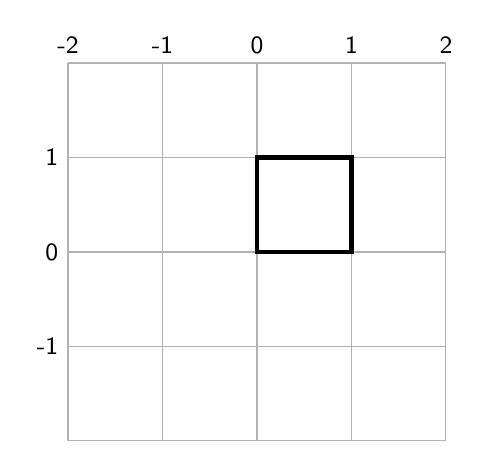
\begin{tikzpicture}[scale=1.2]
        % Draw the background grid: 4 columns (x=-2 to 2) and 3 rows (y=-2 to 1)
        \draw[thin, gray!60] (-2,-2) grid (2,2);
        
        % Horizontal/X-axis labels at the top of each vertical line
        \node[above, font=\small\sffamily] at (-2,2) {-2};
        \node[above, font=\small\sffamily] at (-1,2) {-1};
        \node[above, font=\small\sffamily] at (0,2) {0};
        \node[above, font=\small\sffamily] at (1,2) {1};
        \node[above, font=\small\sffamily] at (2,2) {2};
        
        % Vertical/Y-axis labels next to their respective horizontal lines
        \node[left, font=\small\sffamily] at (-2,1) {1};
        \node[left, font=\small\sffamily] at (-2,0) {0};
        \node[left, font=\small\sffamily] at (-2,-1) {-1};
        
        % Draw the bolded square from (0,0) to (1,1)
        \draw[ultra thick, black] (0,0) rectangle (1,1);
    \end{tikzpicture}
    
    \vspace{0.4cm}
    \flushleft
    View 1: Square with vertices $(0, 0, 0)$, $(1, 0, 0)$, $(1, 1, 0)$, and $(0, 1, 0)$.
  \end{center}


%% ─────────────────────────────────────────────────────────────────────
%% Q21. Square: coordinate matrix, scale (-3/2, 1/2), rotate -60 about z
%% ─────────────────────────────────────────────────────────────────────
\Q{Find the standard matrix for the transformation $T$ on $\mathbb{R}^3$, where $T$ is the composition of a rotation of $-30^\circ$ about the $x$-axis, followed by a contraction with factor $\frac{1}{4}$, followed by a reflection about the $yz$-plane, followed by an orthogonal projection on the $xz$-plane.
\yr{MATH 259 | L-2/T-1 | 2021-22} \mk{15}}

%% ─────────────────────────────────────────────────────────────────────
%% Q: Rot-30x -> Contraction 1/4 -> Reflect yz -> Project xz
%% ─────────────────────────────────────────────────────────────────────
\Q{Describe the geometric effect of multiplying a vector $x$ by $A = \begin{pmatrix} \frac{\sqrt{3}}{2} & -\frac{1}{2} \\ \frac{1}{2} & \frac{\sqrt{3}}{2} \end{pmatrix}$.
\yr{MATH 259 | L-2/T-1 | 2020-21} \mk{10}}


%% ─────────────────────────────────────────────────────────────────────
%% Q14. Geometric effect of A=[[sqrt3/2,-1/2],[1/2,sqrt3/2]]
%% ─────────────────────────────────────────────────────────────────────
\Q{Determine whether $T: M_{nn} \to \mathbb{R}$, where $T(A) = \mathrm{tr}(A)$, is a linear transformation.
\yr{MATH 259 | L-2/T-1 | 2020-21} \mk{10}}

%% ─────────────────────────────────────────────────────────────────────
%% Q15. T(A) = tr(A): Is T:M_nn->R linear?
%% ─────────────────────────────────────────────────────────────────────
\Q{Describe the kernel and range of the orthogonal projection on the plane $y = x$.
\yr{MATH 259 | L-2/T-1 | 2020-21} \mk{10}
\variant{MATH 247 | 2018-19; MATH 143 | 2021-22}}


%% ─────────────────────────────────────────────────────────────────────
%% Q16. Kernel and range of orthogonal projection on plane y=x (in R^3)
%% ─────────────────────────────────────────────────────────────────────
\Q{Find the standard matrix for the composition $T$ on $\mathbb{R}^3$: rotation of $60^\circ$ about the $z$-axis, followed by a reflection about the $xy$-plane, followed by a contraction with factor $k = \frac{1}{2}$. Find the image of $(2,1,-1)$ and explain geometrically.
\yr{MATH 247 | L-2/T-2 | 2020-21} \mk{16}}


%% ─────────────────────────────────────────────────────────────────────
%% Q28. Rot 60 about z -> Reflect xy -> Contraction k=1/2. Find T(2,1,-1).
%% ─────────────────────────────────────────────────────────────────────
%% ─────────────────────────────────────────────────────────────────────
%% CORRECTED Q28. Rot 60 about z -> Reflect xy -> Contraction k=1/2.
%% ─────────────────────────────────────────────────────────────────────
\Q{Let $T_1(x_1,x_2,x_3) = (4x_1, -2x_1+x_2, -x_1-3x_2)$ and $T_2(x_1,x_2,x_3) = (x_1+2x_2, -x_3, 4x_1-x_3)$. Find the standard matrices for $T_1$ and $T_2$. Also find $T_2 \circ T_1$ and $T_1 \circ T_2$.
\yr{MATH 247 | L-2/T-2 | 2020-21} \mk{14.67}}


%% ─────────────────────────────────────────────────────────────────────
%% Q29. T1(x1,x2,x3)=(4x1,-2x1+x2,-x1-3x2) and T2(x1,x2,x3)=(x1+2x2,-x3,4x1-x3).
%%      Standard matrices + T2∘T1 and T1∘T2.
%% ─────────────────────────────────────────────────────────────────────
\Q{Find the standard matrix for $T$ on $\mathbb{R}^3$, where $T$ is a rotation of $60^\circ$ about the $y$-axis, followed by a reflection about the $yz$-plane, followed by a dilation with factor $k = 2$. Find $T(2,-1,4)$.
\yr{MATH 247 | L-2/T-2 | 2019-20} \mk{16.67}}

%% ─────────────────────────────────────────────────────────────────────
%% Q26. Rot 60 about y -> Reflect yz -> Dilation k=2. Find T(2,-1,4).
%% ─────────────────────────────────────────────────────────────────────
\Q{Let $T: \mathbb{R}^4 \to \mathbb{R}^3$ defined by $T(x,y,z,t) = (x-y+z+t,\; x+2z-t,\; x+y+3z-3t)$. Find basis and dimension of $\mathrm{Range}(T)$ and $\ker(T)$.
\yr{MATH 247 | L-2/T-2 | 2019-20} \mk{16.67}
\variant{MATH 243 | 2010-11; MATH 247 | 2018-19}}


%% ─────────────────────────────────────────────────────────────────────
%% Q27. T:R^4->R^3, T(x,y,z,t)=(x-y+z+t, x+2z-t, x+y+3z-3t). ker, Range.
%%      (Same as Q22 but asked in MATH 247 context)
%% ─────────────────────────────────────────────────────────────────────
%% ─────────────────────────────────────────────────────────────────────
%% CORRECTED Q27. T:R^4->R^3, T(x,y,z,t)=(x-y+z+t, x+2z-t, x+y+3z-3t).
%% ─────────────────────────────────────────────────────────────────────
\Q{Determine whether $T(x,y,s,t) = (4x+y-2s-3t,\; 2x+y+s-4t,\; 6x-9s+9t)$ is a linear operator. Find basis and dimension of $\ker T$ and $\mathrm{Range}\,T$.
\yr{MATH 259 | L-2/T-1 | 2018-19} \mk{20}
\variant{MATH 259 | 2014-15, 2021-22; MATH 143 | 2022-23}}


%% ─────────────────────────────────────────────────────────────────────
%% Q10. T(x,y,s,t)=(4x+y-2s-3t, 2x+y+s-4t, 6x-9s+9t): ker, Range
%% ─────────────────────────────────────────────────────────────────────
\Q{Let $T: P_2 \to P_3$ be the linear transformation $T(p(x)) = x p(3x-5)$. Find the matrix for $T$ with respect to the standard bases $B = \{1,x,x^2\}$ and $B' = \{1,x,x^2,x^3\}$. Verify $[T]_{B',B}[x]_B = [T(x)]_{B'}$.
\yr{MATH 259 | L-2/T-1 | 2018-19} \mk{15}
\variant{MATH 215 | 2016-17}}


%% ─────────────────────────────────────────────────────────────────────
%% Q11. T:P2->P3, T(p(x))=x*p(3x-5). Matrix + verify A[p]_B=[T(p)]_{B'}
%% ─────────────────────────────────────────────────────────────────────
\Q{Find the standard matrix for $T$ on $\mathbb{R}^3$, where $T$ is the composition of a reflection about the $xy$-plane, followed by a reflection about the $xz$-plane, followed by an orthogonal projection on the $yz$-plane.
\yr{MATH 259 | L-2/T-1 | 2018-19} \mk{17}}

%% ─────────────────────────────────────────────────────────────────────
%% Q12. Composition: Reflect xy -> Reflect xz -> Project yz
%% ─────────────────────────────────────────────────────────────────────
\Q{Determine whether the linear operator $T: \mathbb{R}^3 \to \mathbb{R}^3$ defined by $w_1 = x_1 + 4x_2 - x_3$, $w_2 = 2x_1 + 7x_2 + x_3$, $w_3 = x_1 + 3x_2$ is one-to-one. If so, find the standard matrix for the inverse operator and find $T^{-1}$.
\yr{MATH 259 | L-2/T-1 | 2018-19} \mk{18}}

%% ─────────────────────────────────────────────────────────────────────
%% Q13. T:R^3->R^3, w1=x1+4x2-x3, w2=2x1+7x2+x3, w3=x1+3x2.
%%     One-to-one? T^-1?
%% ─────────────────────────────────────────────────────────────────────
\Q{Consider the basis $S = \{v_1, v_2, v_3\}$ for $\mathbb{R}^3$, where $v_1 = (1,2,1)$, $v_2 = (2,9,0)$, $v_3 = (3,3,4)$. Let $T: \mathbb{R}^3 \to \mathbb{R}^2$ with $T(v_1) = (1,0)$, $T(v_2) = (-1,1)$, $T(v_3) = (0,1)$. Find a formula for $T(x,y,z)$ and compute $T(7,-3,5)$.
\yr{MATH 247 | L-2/T-2 | 2018-19} \mk{20}}

%% ─────────────────────────────────────────────────────────────────────
%% Q: T:R^3->R^2, basis S={v1=(1,2,1),v2=(2,9,0),v3=(3,3,4)}.
%%    T(v1)=(1,0), T(v2)=(-1,1), T(v3)=(0,1). Find formula, compute T(7,-3,5).
%% ─────────────────────────────────────────────────────────────────────
\Q{Let the linear transformation be defined by $T(x,y,z) = (x-y-3z,\; 5x+6y-4z,\; 7x+4y+2z)$. Find (i) a basis and dimension of $\mathrm{Range}(T)$, (ii) a basis and dimension of $\ker(T)$. Verify the dimension theorem.
\yr{MATH 215 | L-2/T-2 | 2018-19} \mk{30}}

%% ─────────────────────────────────────────────────────────────────────
%% Q: T(x,y,z)=(x-y-3z,5x+6y-4z,7x+4y+2z). Range, ker, dim theorem.
%% ─────────────────────────────────────────────────────────────────────
\Q{Let $S = \{v_1, v_2, v_3\}$ be a basis for $P_2(x)$ where $v_1 = 1 + 2x + x^2$, $v_2 = 2 + 9x$, $v_3 = 3 + 3x + 4x^2$. Find the coordinate vector of $p(x) = 6 + 6x + 3x^2$ relative to $S$.
\yr{MATH 247 | 2018--19}}


%% ─────────────────────────────────────────────────────────────────────
%% Q: S={1+2x+x^2, 2+9x, 3+3x+4x^2} basis for P_2(x).
%%    Find coord vector of p(x)=6+6x+3x^2 relative to S.
%% ─────────────────────────────────────────────────────────────────────
\Q{Let $T: \mathbb{R}^4 \to \mathbb{R}^3$ be the linear transformation defined by $T(x,y,s,t) = (4x + y - 2s - 3t,\; 2x + y + s - 4t,\; 6x - 9s + 9t)$. Find a basis and the dimension of (i) the Kernel of $T$ and (ii) the Range of $T$.
\yr{MATH 259 | 2018--19, 2022--23 (BUET)}}


%% ─────────────────────────────────────────────────────────────────────
%% Q: T:R4->R3, T(x,y,s,t)=(4x+y-2s-3t,2x+y+s-4t,6x-9s+9t).
%%    Basis for ker(T) and range(T). [Same as Q10]
%% ─────────────────────────────────────────────────────────────────────
\Q{Determine whether the linear operator $T: \mathbb{R}^3 \to \mathbb{R}^3$ defined by $w_1 = x_1 + 2x_2 + x_3$, $w_2 = -2x_1 + x_2 + 4x_3$, $w_3 = 7x_1 + 4x_2 - 5x_3$ is one-to-one. If so, find the inverse standard matrix and $T^{-1}$.
\yr{MATH 259 | L-2/T-1 | 2017-18} \mk{17}}

%% ─────────────────────────────────────────────────────────────────────
%% Q34. T: w1=x1+2x2+x3, w2=-2x1+x2+4x3, w3=7x1+4x2-5x3.
%%      One-to-one? If so, T^-1?
%% ─────────────────────────────────────────────────────────────────────
\Q{If $T: V \to W$ is a linear transformation, prove that (i) the kernel of $T$ is a subspace of $V$; (ii) the range of $T$ is a subspace of $W$.
\yr{MATH 247 | L-2/T-2 | 2017-18} \mk{16.67}}

%% ─────────────────────────────────────────────────────────────────────
%% Q: Kernel and Range of linear transformation T: V -> W
%% ─────────────────────────────────────────────────────────────────────
\Q{Let $v_1 = \begin{pmatrix} 1 \\ 3 \end{pmatrix}$ and $v_2 = \begin{pmatrix} -1 \\ 4 \end{pmatrix}$, and let $A = \begin{pmatrix} 1 & 3 \\ -2 & 5 \end{pmatrix}$ be the matrix for $T: \mathbb{R}^2 \to \mathbb{R}^2$ with respect to the basis $B = \{v_1, v_2\}$. (i) Find $[T(v_1)]_B$ and $[T(v_2)]_B$. (ii) Find $T(v_1)$ and $T(v_2)$. (iii) Find a formula for $T\begin{pmatrix} x_1 \\ x_2 \end{pmatrix}$. (iv) Compute $T\begin{pmatrix} 1 \\ 1 \end{pmatrix}$.
\yr{MATH 247 | L-2/T-2 | 2017-18} \mk{20}}

%% ─────────────────────────────────────────────────────────────────────
%% Q35. T:R^2->R^2 via matrix A=[[1,3],[-2,5]] relative to B={v1,v2}.
%%      v1=(1,3), v2=(-1,4). Find formula for T, compute T(1,1).
%% ─────────────────────────────────────────────────────────────────────
\Q{Let $T: \mathbb{R}^4 \to \mathbb{R}^3$ defined by $T(w,x,y,z) = (2w+4x+6y+5z,\; -w-2x+2y,\; 8y+4z)$. Find a basis for (i) the kernel of $T$ and (ii) the range of $T$.
\yr{MATH 215 | L-2/T-2 | 2017-18} \mk{17}}

%% ─────────────────────────────────────────────────────────────────────
%% Q: T:R^4->R^3, T(w,x,y,z)=(2w+4x+6y+5z,-w-2x+2y,8y+4z).
%%    Basis for ker(T) and range(T).
%% ─────────────────────────────────────────────────────────────────────
\Q{Let $B = \{(1,3),(-2,-2)\}$ and $B' = \{(-12,0),(-4,4)\}$ be two bases for $\mathbb{R}^2$, and let $A = \begin{pmatrix} 3 & 2 \\ 0 & 4 \end{pmatrix}$ be the matrix for $T: \mathbb{R}^2 \to \mathbb{R}^2$ relative to $B$. (i) Find transition matrix $P$ from $B'$ to $B$. (ii) Find $[v]_B$ and $[T(v)]_B$ where $[v]_{B'} = \begin{pmatrix} -1 \\ 2 \end{pmatrix}$. (iii) Find $A'$ and $P^{-1}$. (iv) Find $[T(v)]_{B'}$.
\yr{MATH 215 | L-2/T-2 | 2017-18} \mk{20}}

%% ─────────────────────────────────────────────────────────────────────
%% Q: Transition matrix B->B'. B={(1,3),(-2,-2)}, B'={(-12,0),(-4,4)}.
%%    A=[[3,2],[0,4]] relative to B. [v]_{B'}=(-1,2).
%% ─────────────────────────────────────────────────────────────────────
\Q{Let $T: \mathbb{R}^3 \to \mathbb{R}^3$ be the linear operator defined by $T(x,y,z) = (x+2y-z,\; 2x+y+z,\; y+z)$. Find the rank and nullity of $T$.
\yr{MATH 247 | L-2/T-2 | 2017-18} \mk{15}}


%% ─────────────────────────────────────────────────────────────────────
%% Q: T(x,y,z)=(x+2y-z,2x+y+z,y+z). Find rank and nullity.
%% ─────────────────────────────────────────────────────────────────────
\Q{Determine whether the mapping $T: \mathbb{R}^3 \to \mathbb{R}^3$ defined by $T(x,y,z) = (x+2y-z,\; y+z,\; x+y-2z)$ is a linear operator. If so, find the basis and dimension of (i) $\mathrm{Im}\,T$ and (ii) $\ker T$.
\yr{MATH 247 | L-2/T-2 | 2017-18} \mk{15}}

%% ─────────────────────────────────────────────────────────────────────
%% Q: T(x,y,z)=(x+2y-z,y+z,x+y-2z): linear? Im(T), ker(T).
%%    (Similar to Q4 but slightly different — same matrix!)
%% ─────────────────────────────────────────────────────────────────────
\Q{Find eigenvalues and corresponding eigenvectors of the linear transformation $T$ on $\mathbb{R}^3$ defined by the reflection about the $zx$-plane. Is the transformation one-to-one?
\yr{MATH 259 | L-2/T-1 | 2017-18} \mk{10}}

%% ─────────────────────────────────────────────────────────────────────
%% Q: Reflection about zx-plane. Eigenvalues, eigenvectors, one-to-one?
%% ─────────────────────────────────────────────────────────────────────
\Q{Find the standard matrix for the transformation $T$ on $\mathbb{R}^3$, where $T$ is the composition of a counterclockwise rotation of $\frac{\pi}{3}$ about the $y$-axis, followed by a reflection about the $yz$-plane, followed by contraction with factor $\frac{1}{2}$. Then find the image of $(2,0,3)$.
\yr{MATH 215 | L-2/T-2 | 2017-18} \mk{15}}

%% ─────────────────────────────────────────────────────────────────────
%% Q: Rot pi/3 about y -> Reflect yz -> Contraction 1/2. Image of (2,0,3).
%% ─────────────────────────────────────────────────────────────────────
\Q{Let $v_1 = \begin{pmatrix}1\\3\end{pmatrix}$ and $v_2 = \begin{pmatrix}-1\\4\end{pmatrix}$, and let $A = \begin{pmatrix}1 & 3\\ -2 & 5\end{pmatrix}$ be the matrix for $T: \mathbb{R}^2 \to \mathbb{R}^2$ relative to basis $B = \{v_1, v_2\}$. (i) Find $[T(v_1)]_B$ and $[T(v_2)]_B$. (ii) Find $T(v_1)$ and $T(v_2)$. (iii) Find a formula for $T(x_1,x_2)^T$. (iv) Compute $T(1,1)^T$.
\yr{MATH 247 | 2017--18}}

%% ─────────────────────────────────────────────────────────────────────
%% Q: v1=(1,3), v2=(-1,4), A=[[1,3],[-2,5]] matrix of T rel to B.
%%    Find [T(v1)]_B, [T(v2)]_B, T(v1), T(v2), formula, T(1,1).
%%    [Same as Q35]
%% ─────────────────────────────────────────────────────────────────────
%% ══════════════════════════════════════════════════════════════════════
%%  SECTION 7: COMPLEX VECTORS
%% ══════════════════════════════════════════════════════════════════════
\Q{Derive the standard matrices for the operations on $\mathbb{R}^3$: a rotation of $45^\circ$ about the $y$-axis, followed by an orthogonal projection on the $yz$-plane, followed by a dilation with $k = 2$. Find the standard matrix for the composition and the image of $(-1,-2,3)$. Is the operator one-to-one?
\yr{MATH 259 | L-2/T-1 | 2016-17} \mk{20}}


%% ─────────────────────────────────────────────────────────────────────
%% Q33. Rot 45 about y -> Project yz -> Dilation k=2. Image of (-1,-2,3). One-to-one?
%% ─────────────────────────────────────────────────────────────────────
\Q{Find the standard matrix for the linear operator $T: \mathbb{R}^3 \to \mathbb{R}^3$ given by $w_1 = 3x+5y-z$, $w_2 = 4x-y+z$, $w_3 = 3x+2y-z$. Then calculate $T(-1,2,4)$.
\yr{MATH 215 | L-2/T-2 | 2016-17} \mk{15}}


%% ─────────────────────────────────────────────────────────────────────
%% Q: Standard matrix for w1=3x+5y-z, w2=4x-y+z, w3=3x+2y-z. Find T(-1,2,4).
%% ─────────────────────────────────────────────────────────────────────
\Q{Let $T: P_2 \to P_3$ be the linear transformation defined by $T(a+bx+cx^2) = x\bigl(a + b(x-3) + c(x-3)^2\bigr)$. Find the matrix for $T$ with respect to $E = \{1,x,x^2\}$ and $E' = \{1,x,x^2,x^3\}$. Verify $A[p]_E = [T(p)]_{E'}$.
\yr{MATH 215 | L-2/T-2 | 2016-17} \mk{15}}

%% ─────────────────────────────────────────────────────────────────────
%% Q: T:P2->P3, T(a+bx+cx^2) = x(a+b(x-3)+c(x-3)^2).
%%    Matrix w.r.t. E={1,x,x^2} and E'={1,x,x^2,x^3}. Verify A[p]_E=[T(p)]_{E'}.
%% ─────────────────────────────────────────────────────────────────────
\Q{Consider the basis $S = \{v_1, v_2, v_3\}$ for $\mathbb{R}^3$, where $v_1 = (1,1,1)$, $v_2 = (1,1,0)$, $v_3 = (1,0,0)$. Let $T: \mathbb{R}^3 \to \mathbb{R}^2$ with $T(v_1) = (1,0)$, $T(v_2) = (2,-1)$, $T(v_3) = (4,3)$. Find a formula for $T(x_1,x_2,x_3)$ and compute $T(5,-3,2)$.
\yr{MATH 259 | L-2/T-1 | 2015-16} \mk{15}
\variant{MATH 259 | 2014-15, 2020-21, 2021-22; MATH 215 | 2016-17; MATH 143 | 2021-22, 2022-23}}


%% ─────────────────────────────────────────────────────────────────────
%% Q8. T:R^3->R^2 defined by values on basis S={v1,v2,v3}
%%     v1=(1,1,1), v2=(1,1,0), v3=(1,0,0)
%%     T(v1)=(1,0), T(v2)=(2,-1), T(v3)=(4,3). Find T(5,-3,2).
%% ─────────────────────────────────────────────────────────────────────
\Q{Let $T$ be multiplication by $A = \begin{pmatrix} 4 & 1 & 5 & 2 \\ 1 & 2 & 3 & 0 \end{pmatrix}$. Find a basis for $\mathrm{Range}(T)$, $\ker(T)$, the rank and nullity of $T$.
\yr{MATH 259 | L-2/T-1 | 2015-16} \mk{10}
\variant{MATH 259 | 2014-15, 2018-19, 2021-22}}


%% ─────────────────────────────────────────────────────────────────────
%% Q9. T = multiplication by A=[[4,1,5,2],[1,2,3,0]].
%%     Range, ker, rank, nullity.
%% ─────────────────────────────────────────────────────────────────────
\Q{Let $l$ be the line in the $xy$-plane through the origin making angle $\theta$ with the positive $x$-axis ($0 \le \theta < \pi$). Let $T: \mathbb{R}^2 \to \mathbb{R}^2$ map each vector to its orthogonal projection on $l$. (i) Find the standard matrix for $T$. (ii) Find the projection of $X = (2,5)$ onto the line with $\theta = \pi/3$.
\yr{MATH 259 | L-2/T-1 | 2015-16} \mk{15}}

%% ─────────────────────────────────────────────────────────────────────
%% Q30. Orthogonal projection on line at angle theta.
%%      Project X=(2,5) onto line at theta=pi/3.
%% ─────────────────────────────────────────────────────────────────────
\Q{Determine whether multiplication by $A = \begin{pmatrix} 1 & -1 \\ 2 & 0 \\ 3 & -4 \end{pmatrix}$ is one-to-one. Explain.
\yr{MATH 259 | L-2/T-1 | 2015-16} \mk{10}}

%% ─────────────────────────────────────────────────────────────────────
%% Q31. T = multiplication by A=[[1,-1],[2,0],[3,-4]]. One-to-one?
%% ─────────────────────────────────────────────────────────────────────
\Q{Find the eigenvalues and corresponding eigenvectors of $T: \mathbb{R}^2 \to \mathbb{R}^2$ where $T$ is the reflection about the line $y = x$. Check your conclusion from the standard matrix.
\yr{MATH 259 | L-2/T-1 | 2015-16} \mk{10}}


%% ─────────────────────────────────────────────────────────────────────
%% Q32. T = reflection about y=x in R^2. Eigenvalues/eigenvectors.
%% ─────────────────────────────────────────────────────────────────────
\Q{Find the standard matrix for the composition in $\mathbb{R}^3$: a rotation of $30^\circ$ about the $y$-axis, followed by a reflection about the $xy$-plane, followed by an orthogonal projection on the $yz$-plane. Find the image of $(-1,2,3)$.
\yr{MATH 243 | L-2/T-2 | 2015-16} \mk{15}
\variant{MATH 247 | 2019-20; MATH 143 | 2022-23}}

%% ─────────────────────────────────────────────────────────────────────
%% Q: Compose Rot30y -> Reflect xy -> Project yz. Image of (-1,2,3).
%% ─────────────────────────────────────────────────────────────────────
\Q{Let $T: \mathbb{R}^3 \to \mathbb{R}^3$ be the linear operator defined by $T(x,y,z) = (x+2y,\; y-z,\; x+2z)$. Find the rank and nullity of $T$. Hence verify the Dimension Theorem.
\yr{MATH 247 | L-2/T-2 | 2015-16} \mk{15}}

%% ─────────────────────────────────────────────────────────────────────
%% Q: T(x,y,z)=(x+2y,y-z,x+2z). Rank, nullity, verify Dimension Theorem.
%% ─────────────────────────────────────────────────────────────────────
\Q{Let $T: \mathbb{R}^3 \to \mathbb{R}^3$ be a linear transformation where $T(x,y,z) = (x+2y+z,\; y+z,\; x+y-2z)$. Find the basis of $\mathrm{Im}(T)$ and $\ker(T)$. Also find rank and nullity of $T$.
\yr{MATH 247 | L-2/T-2 | 2014-15} \mk{15}}

%% ─────────────────────────────────────────────────────────────────────
%% Q: T(x,y,z)=(x+2y+z,y+z,x+y-2z). Im(T), ker(T), rank, nullity.
%% ─────────────────────────────────────────────────────────────────────
\Q{Derive the standard matrices for the operations on $\mathbb{R}^3$: a rotation of $-30^\circ$ about the $x$-axis, followed by a reflection about the $yz$-plane, followed by an orthogonal projection on the $zx$-plane. Find the standard matrix and the image of the triangle with vertices $(-1,2,-3)$, $(1,-2,-3)$, $(-1,-2,3)$.
\yr{MATH 259 | L-2/T-1 | 2013-14} \mk{20}
\variant{MATH 259 | 2014-15, 2016-17, 2017-18, 2018-19, 2021-22}}

%% ─────────────────────────────────────────────────────────────────────
%% Q6. Compose: Rot -30 x-axis -> Reflect yz -> Project zx.
%%     Image of triangle (-1,2,-3),(1,-2,-3),(-1,-2,3)
%% ─────────────────────────────────────────────────────────────────────
\Q{Determine the eigenvalues and corresponding eigenvectors of $T: \mathbb{R}^3 \to \mathbb{R}^3$ defined as reflection about the $yz$-plane. Check your conclusion by computing from the standard matrix.
\yr{MATH 259 | L-2/T-1 | 2013-14} \mk{10}
\variant{MATH 259 | 2014-15, 2017-18}}

%% ─────────────────────────────────────────────────────────────────────
%% Q7. Eigenvalues/eigenvectors of T = reflection about yz-plane
%% ─────────────────────────────────────────────────────────────────────
\Q{Let $T: P_2 \to P_3$ be the linear transformation defined by $T(p(x)) = x \cdot p(x-3)$. Find the matrix for $T$ with respect to the standard bases $B = \{1, x, x^2\}$ and $B' = \{1, x, x^2, x^3\}$. Verify the relation $A[p]_B = [T(p)]_{B'}$.
\yr{MATH 243 | L-2/T-2 | 2013-14} \mk{15}
\variant{MATH 215 | 2016-17}}

%% ─────────────────────────────────────────────────────────────────────
%% Q: T:P2->P3, T(p(x))=x*p(x-3). Matrix + verify A[p]_B=[T(p)]_{B'}.
%% ─────────────────────────────────────────────────────────────────────
\Q{(a) Determine whether the function 
$T : M_{22} \rightarrow \Re$ defined by $T\left(\begin{bmatrix} a & b \\ c & d \end{bmatrix}\right) = 3a - 4b + c - d$
is linear transformation or not. Justify your answer. \mk{10}

(b) If $T : V \rightarrow W$ is linear transformation, then prove that 
(i) The kernel of $T$ is a subspace of $V$ and (ii) The range of $T$ is a subspace of $W$. \mk{15}
\yr{MATH 259 | L-2/T-1 | 2013-14}
}

%% ── Answer: Linear Transformation, Kernel, and Range Subspaces ────────
\Q{Let $F: \mathbb{R}^3 \to \mathbb{R}^3$ be defined by $F(x,y,z) = (x+2y-3z,\; 2x+5y-4z,\; x+4y+z)$. Find a basis and dimension of the kernel and image of $F$.
\yr{MATH 243 | L-2/T-2 | 2012-13} \mk{15}}

%% ─────────────────────────────────────────────────────────────────────
%% Q: F(x,y,z)=(x+2y-3z,2x+5y-4z,x+4y+z). Kernel and Image.
%% ─────────────────────────────────────────────────────────────────────
\Q{Consider the basis $S = \{u, v, w\}$ for $\mathbb{R}^3$, where $u = (1,1,1)$, $v = (1,1,0)$, $w = (1,0,0)$. Let $T: \mathbb{R}^3 \to \mathbb{R}^3$ with $T(u) = (2,-1,4)$, $T(v) = (3,0,1)$, $T(w) = (-1,5,1)$. Find a formula for $T(x,y,z)$ and compute $T(2,-3,5)$.
\yr{MATH 243 | L-2/T-2 | 2011-12} \mk{15}
\variant{MATH 243 | 2016-17}}

%% ─────────────────────────────────────────────────────────────────────
%% Q: T:R^3->R^3, S={u=(1,1,1),v=(1,1,0),w=(1,0,0)}.
%%    T(u)=(2,-1,4), T(v)=(3,0,1), T(w)=(-1,5,1). Find formula, T(2,-3,5).
%% ─────────────────────────────────────────────────────────────────────
\secdivider{Complex Vectors}{Hermitian, Skew-Hermitian, Unitary Matrices, Spectral Theorem}{cG}{pink!60!red}

\markboth{S7: Complex Vectors}{S7: Complex Vectors}
\label{sec:S7}
\section*{S7 \quad Complex Vectors}
\addcontentsline{toc}{section}{S7: Complex Vectors}

\Q{Define Hermitian and skew-Hermitian matrices. Examine whether the eigenvalues of the Hermitian matrix $H = \begin{pmatrix} 3 & 2-3i \\ 2+3i & -1 \end{pmatrix}$ are real. If so, verify that eigenvectors from different eigenspaces are orthogonal.
\yr{MATH 143 | L-1/T-2 | 2023-24} \mk{12}}

%% ─────────────────────────────────────────────────────────────────────
%% Q1. Define Hermitian/skew-Hermitian; H=[[3,2-3i],[2+3i,-1]]
%%     eigenvalues real; eigenvectors orthogonal
%% ─────────────────────────────────────────────────────────────────────
\Q{Find the singular value decomposition (SVD) of $A = \begin{pmatrix} 1 & 1 \\ 0 & 1 \\ 1 & 0 \end{pmatrix}$.
\yr{MATH 143 | L-1/T-2 | 2023-24, 2021--22} \mk{12}
\variant{MATH 143 | 2022-23}}


%% ─────────────────────────────────────────────────────────────────────
%% Q8. SVD of A = [[1,1],[0,1],[1,0]]
%% ─────────────────────────────────────────────────────────────────────
\Q{Show that the Hermitian matrix $A = \begin{pmatrix} 2 & 1+i \\ 1-i & 3 \end{pmatrix}$ has real eigenvalues and that eigenvectors from different eigenspaces are orthogonal.
\yr{MATH 143 | L-1/T-2 | 2022-23} \mk{12}}

%% ─────────────────────────────────────────────────────────────────────
%% Q3. A=[[2,1+i],[1-i,3]] real eigenvalues + orthogonal eigenvectors
%% ─────────────────────────────────────────────────────────────────────
\Q{Find a singular value decomposition (SVD) of the matrix $A = \begin{pmatrix} 1 & 0 & -1 \\ 1 & 1 & 1 \end{pmatrix}$.
\yr{MATH 143 | L-1/T-2 |} \mk{17}}
 
%% ─────────────────────────────────────────────────────────────────────
%% Q9. SVD of A = [[1,0,-1],[1,1,1]]
%% ─────────────────────────────────────────────────────────────────────
\Q{Find a matrix $P$ that unitarily diagonalizes the Hermitian matrix $A = \begin{pmatrix} 2 & 1+i \\ 1-i & 3 \end{pmatrix}$. Verify that $P^* AP$ is a diagonal matrix.
\yr{MATH 143 | L-1/T-2 | 2021-22} \mk{12}}

%% ─────────────────────────────────────────────────────────────────────
%% Q6. Unitarily diagonalize A=[[2,1+i],[1-i,3]]; verify P*AP diagonal
%% ─────────────────────────────────────────────────────────────────────
\Q{Define Hermitian and Skew-Hermitian matrices with examples. Prove that any square matrix can be uniquely expressed as the sum of a symmetric and a skew-symmetric matrix. Verify for $A = \begin{pmatrix} i & 2-3i & 4+5i \\ 6+i & 0 & 4-5i \\ -i & 2-i & 2+i \end{pmatrix}$.
\yr{MATH 259 | L-2/T-1 | 2020-21} \mk{18}}

%% ─────────────────────────────────────────────────────────────────────
%% Q5. Define H/sH matrices; prove unique decomp; verify for 3x3
%% ─────────────────────────────────────────────────────────────────────
\Q{Define orthogonal matrix and unitary matrix with examples. Express \\$A = \begin{pmatrix} -2+3i & 1-i & 2+i \\ 3 & 4-5i & 5 \\ 1 & 1+i & -2+2i \end{pmatrix}$ as a sum of Hermitian and skew-Hermitian matrices.
\yr{MATH 259 | L-2/T-1 | 2017-18} \mk{15}}

%% ─────────────────────────────────────────────────────────────────────
%% Q4. Define orthogonal/unitary matrices; A (3x3 complex) = H + K
%% ─────────────────────────────────────────────────────────────────────
\Q{Prove that every square matrix can be uniquely expressed as $P + iQ$, where $P$ and $Q$ are Hermitian matrices.
\yr{MATH 259 | L-2/T-1 | 2016-17} \mk{10}
\variant{MATH 259 | 2017-18, 2020-21}}

%% ─────────────────────────────────────────────────────────────────────
%% Q2. Prove every square matrix = P + iQ, P,Q Hermitian
%% ─────────────────────────────────────────────────────────────────────
\Q{Define Hermitian matrix and skew-Hermitian matrix with examples. Prove that every square matrix can be uniquely expressed as $P + iQ$, where $P$ and $Q$ are Hermitian matrices.
\yr{MATH 259 | L-2/T-1 | 2016-17} \mk{10}
\variant{MATH 259 | 2017-18, 2020-21}}


%% ─────────────────────────────────────────────────────────────────────
%% Q5. Hermitian + skew-Hermitian decomposition proof
%% ─────────────────────────────────────────────────────────────────────
\end{document}